\documentclass[12pt,a4paper,oneside]{article}
\usepackage[QX]{polski}
\usepackage[T1]{fontenc}
\usepackage[utf8]{inputenc}
\usepackage{latexsym}
\usepackage{tgpagella}
\usepackage{lmodern}
\usepackage{amsmath,amsthm,amsfonts,amssymb,alltt}
\usepackage{epsfig}
\usepackage{pdflscape}
\usepackage{caption}
\usepackage{indentfirst}
\usepackage{float}
%\usepackage{showkeys}
\bibliographystyle{plabbrv}


\usepackage{color}
\usepackage[polish]{babel}
\usepackage{datetime2}
\usepackage[x11names,dvipsnames,table]{xcolor}
\usepackage{hyperref}
\hypersetup{
pdfauthor={Roman Czapla, Olaf Bar},
colorlinks=True,
linkcolor=darkgray,  % color of internal links (change box color with linkbordercolor)
citecolor=BrickRed,  % color of links to bibliography
filecolor=Magenta,   % color of file links
urlcolor=BlueViolet}	%%pdfpagemode=FullScreen}

% diagramy, grafy itp.
\usepackage{tikz}
\usetikzlibrary{positioning}
\usetikzlibrary{arrows}
\usetikzlibrary{arrows.meta}
\usetikzlibrary{chains,fit,shapes,calc}
\tikzset{main node/.style={circle,fill=blue!20,draw,minimum size=1cm,inner sep=0pt}}

% algorytmy
\usepackage[linesnumbered,lined,commentsnumbered]{algorithm2e}
\SetKwFor{ForEach}{for each}{do}{end for}%
\SetKwFor{ForAll}{for all}{do}{end for}%
\newenvironment{myalgorithm}
{\rule{\textwidth}{0.5mm}\\\SetAlCapSty{}\SetAlgoNoEnd\SetAlgoNoLine\begin{algorithm}}{\end{algorithm}\rule{\textwidth}{0.5mm}}


%---------------------
\overfullrule=2mm
\pagestyle{plain}
\textwidth=15cm \textheight=685pt \topmargin=-25pt \linespread{1.3} 
\setlength{\parskip}{0pt}
\setlength\arraycolsep{2pt}
\oddsidemargin =0.9cm
\evensidemargin =-0.1cm

\captionsetup{width=.95\linewidth, justification=centering}
%---------------------




\newtheorem{tw}{Twierdzenie}[section]
\newtheorem{lem}[tw]{Lemat}
\newtheorem{co}[tw]{Wniosek}
\newtheorem{prop}[tw]{Stwierdzenie}
\theoremstyle{definition}
\newtheorem{ex}{Przykład}
\newtheorem{re}[tw]{Uwaga}
\newtheorem{de}{Definicja}[section]



\newcommand{\bC}{{\mathbb C}}
\newcommand{\bR}{{\mathbb R}}
\newcommand{\bZ}{{\mathbb Z}}
\newcommand{\bQ}{{\mathbb Q}}
\newcommand{\bN}{{\mathbb N}}
\newcommand{\captionT}[1]{\caption{\textsc{\footnotesize{#1}}}}
\renewcommand\figurename{Rys.}

\numberwithin{equation}{section}
\renewcommand{\thefootnote}{\arabic{footnote})}
%\renewcommand{\thefootnote}{\alph{footnote})}



\begin{document}

% --------------------------------------------
% Strona tytułowa
% --------------------------------------------

\thispagestyle{empty}
\begin{titlepage}
\begin{center}\Large
Uniwersytet Komisji Edukacji Narodowej w Krakowie\\
\large
Instytut Bezpieczeństwa i Informatyki\\
\vskip 10pt
\end{center}
\begin{center}
\centering 
\includegraphics[width=1.0\columnwidth]{images/logo.png}
\end{center}

\begin{center}
 {\bf \fontsize{14pt}{14pt}\selectfont PROJEKT INŻYNIERSKI \\ RAPORT Z REALIZACJI PROJEKTU\\
 }
 {\fontsize{12pt}{12pt} raport z okres: 20.10.2024 - 20.01.2025}
\end{center}
\vskip 5pt
\begin{center}
 {\bf \fontsize{12pt}{22pt}\selectfont System rekomendacji produktów. Tworzenie algorytmu rekomendacyjnego na
 podstawie preferencji użytkowników – aplikacja przeglądarkowa}
\end{center}

\begin{center}
 {\fontsize{12pt}{12pt}\selectfont wykonany przez: }
\end{center}
\begin{center}
 {\bf\fontsize{16pt}{16pt}\selectfont Krzysztof Bielkiewicz}\\
 {\fontsize{12pt}{12pt}\selectfont Nr albumu: 156791 \\\&\\}
 {\bf\fontsize{16pt}{16pt}\selectfont Maciej Fabef}\\
 {\fontsize{12pt}{12pt}\selectfont Nr albumu: 156750\\\&\\}
 {\bf\fontsize{16pt}{16pt}\selectfont Grzegorz Golonka }\\
 {\fontsize{12pt}{12pt}\selectfont Nr albumu: 156742}
\end{center}
\begin{center}
 {\fontsize{12pt}{12pt}\selectfont pod opieką:}\\
 {\bf\fontsize{12pt}{12pt}\selectfont dr hab. inż. Mateusz Muchacki, prof. UKEN}
\end{center}

%\mbox{}
\vspace*{\fill}
%\vskip 50pt
\begin{center}
\large
Kraków \the\year\\
(ostatnia aktualizacja: \DTMcurrenttime,\;\today)
\end{center}
\end{titlepage}
\setcounter{page}{0} 
\newpage\null\thispagestyle{empty}
%\setcounter{page}{0} 
%\newpage
%\thispagestyle{empty}

\tableofcontents


\newpage

\section{Informacja na temat postępów prac nad projektem}

\subsection{Zespół projektowy}
\textit{Lista osób tworzących zespół projektowy wraz z danymi kontaktowi (e-mail).}
    \paragraph{Grzegorz Golonka}
    \begin{itemize}
        \item E-mail: grzegorz.golonka@student.up.krakow.pl
    \end{itemize}
    \paragraph{Krzysztof Bielkiewicz}
    \begin{itemize}
        \item E-mail:  krzysztof.bielkiewicz@student.up.krakow.pl
    \end{itemize}
    \paragraph{Maciej Faber}
    \begin{itemize}
        \item E-mail:
    \end{itemize}

\subsection{Zrealizowane zadania}
\textit{Lista zrealizowanych prac z podziałem na członków zespołu projektowego.}
\paragraph{Krzysztof Bielkiewicz}
\begin{itemize}
    \item Zadanie 1. Stworzenie nagłówka dla aplikacji (\hyperref[1.3.1]{sekcja 1.3.1})
    \item Zadanie 2. Stworzenie strony startowej (\hyperref[1.3.2]{sekcja 1.3.2})
    \item Zadanie 3. Opcja wyszukiwania po słowach kluczowych (\hyperref[1.3.3]{sekcja 1.3.3})
    \item Zadanie 4. Opcja wyszukiwania po kategoriach (\hyperref[1.3.4]{sekcja 1.3.4})
    \item Zadanie 5. Stworzenie strony z ulubionymi produktami (\hyperref[1.3.5]{sekcja 1.3.5})
    \item Zadanie 6. Stworzenie strony profilu z opcją edycji (\hyperref[1.3.6]{sekcja 1.3.6})
    \item Zadanie 7. Oprawa graficzna dla strony dodania adresu dostawy (\hyperref[1.3.7]{sekcja 1.3.7})
    \item Zadanie 8. Oprawa graficzna koszyka (\hyperref[1.3.8]{sekcja 1.3.8})
    \item Zadanie 9. Oprawa graficzna wyboru adresu dostawy (\hyperref[1.3.9]{sekcja 1.3.9})
    \item Zadanie 10. Oprawa graficzna dla metod płatności (\hyperref[1.3.10]{sekcja 1.3.10})
    \item Zadanie 11. Oprawa graficzna szczegółów zamówienia (\hyperref[1.3.11]{sekcja 1.3.11})
    \item Zadanie 12. Oprawa graficzna dla listy zamówień (\hyperref[1.3.12]{sekcja 1.3.12})
    \item Zadanie 13. Wyświetlanie produktów z bazy danych (\hyperref[1.3.13]{sekcja 1.3.13})
    \item Zadanie 14. Funckja dodawania produktów do ulubionych (\hyperref[1.3.14]{sekcja 1.3.14})
    \item Zadanie 15. Paginacja produktów na stronach (\hyperref[1.3.15]{sekcja 1.3.15})
    \item Zadanie 16. Oprawa graficzna szczegółów produktu (\hyperref[1.3.16]{sekcja 1.3.16})
    \item Zadanie 17. Custom errory i oprawa graficzna rejestracji (\hyperref[1.3.17]{sekcja 1.3.17})
    \item Zadanie 18. Custom errory i oprawa graficzna loginu (\hyperref[1.3.18]{sekcja 1.3.18})
\end{itemize}
\paragraph{Grzegorz Golonka}
\begin{itemize}
    \item Zadanie nr 1. Utworzenie pliku README.md                          (\ref{section:1.3.19})
    \item zadanie nr 2. Utworzenie modeli bazodanowych                      (\ref{section:1.3.20})
    \item Zadanie nr 3. Dodanie skryptów do inicjalizacji projektu          (\ref{section:1.3.21})
    \item Zadanie nr 4. Stworzenie seeda produktów i kategorii              (\ref{section:1.3.22})
    \item Zadanie nr 5. Formularze do modelów bazodanowych                  (\ref{section:1.3.23})
    \item Zadanie nr 6. Obsługa widoków adresu i listy adresów użytkownika  (\ref{section:1.3.24})
    \item Zadanie nr 7. Obsługa widoków metody płatności i kodu Blik        (\ref{section:1.3.25})
    \item Zadanie nr 8. Weryfikacja danych przy składaniu zamówienia               (\ref{section:1.3.26})
    \item Zadanie nr 9. Tworzenie zamówienia i wysyłanie powiadomień               (\ref{section:1.3.27})
    \item Zadanie nr 10. Implementacja widoku szczegółów zamówienia              (\ref{section:1.3.28})
    \item Zadanie nr 11. Automatyczna aktualizacja statusu zamówienia              (\ref{section:1.3.29})
    \item Zadanie nr 12. Przygotowanie do oceniania produktów w zamówieniu             (\ref{section:1.3.30})
    \item Zadanie nr 13. Automatyczne tworzenie konwersacji przy zamówieniu             (\ref{section:1.3.31})
    \item Zadanie nr 14. Widok listy wiadomości i konwersacji              (\ref{section:1.3.32})
    \item Zadanie nr 15. Obsługa ładowania wiadomości              (\ref{section:1.3.33})
    \item Zadanie nr 16. Utworzenie systemu oceniania produktów             (\ref{section:1.3.34})
    \item Zadanie nr 17. Integracja systemu ocen z widokiem produktu            (\ref{section:1.3.35})
    \item Zadanie nr 18.  Dynamiczna obsługa ocen i ich edycji             (\ref{section:1.3.36})

\end{itemize}
\paragraph{Maciej Faber}
\begin{itemize}
\item zadanie nr 1 (sekcja 1.3.m+1)
\item zadanie nr 2 (sekcja 1.3.m+2)
\item \dots
\item zadanie nr k (sekcja 1.3.m+k)

\end{itemize}

\subsection {Opis zrealizowanych prac}
\subsubsection{Krzysztof Bielkiewicz: Stworzenie nagłówka dla aplikacji}
\label{1.3.1}
\textit{Responsywny nagłówek dla całej aplikacji, zawierający:}
\begin{itemize}
    \item Nazwe aplikacji, funkcje wyszukiwania
    \item Przycisk z wyborem kategorii i przekierowania do produktów z wybranej kategorii
    \item Przyciski przekierowania do strony z Ulubione i Koszyka
    \item Przycisk Profile pokazujący przyciski przekierowujące do:
        \begin{itemize}
            \item Edycji profilu, Dodania adresu
            \item Wiadomości, Szczegółów zamówienia
            \item Wylogowania
        \end{itemize}
\end{itemize}

\begin{figure}[H]
    \centering
    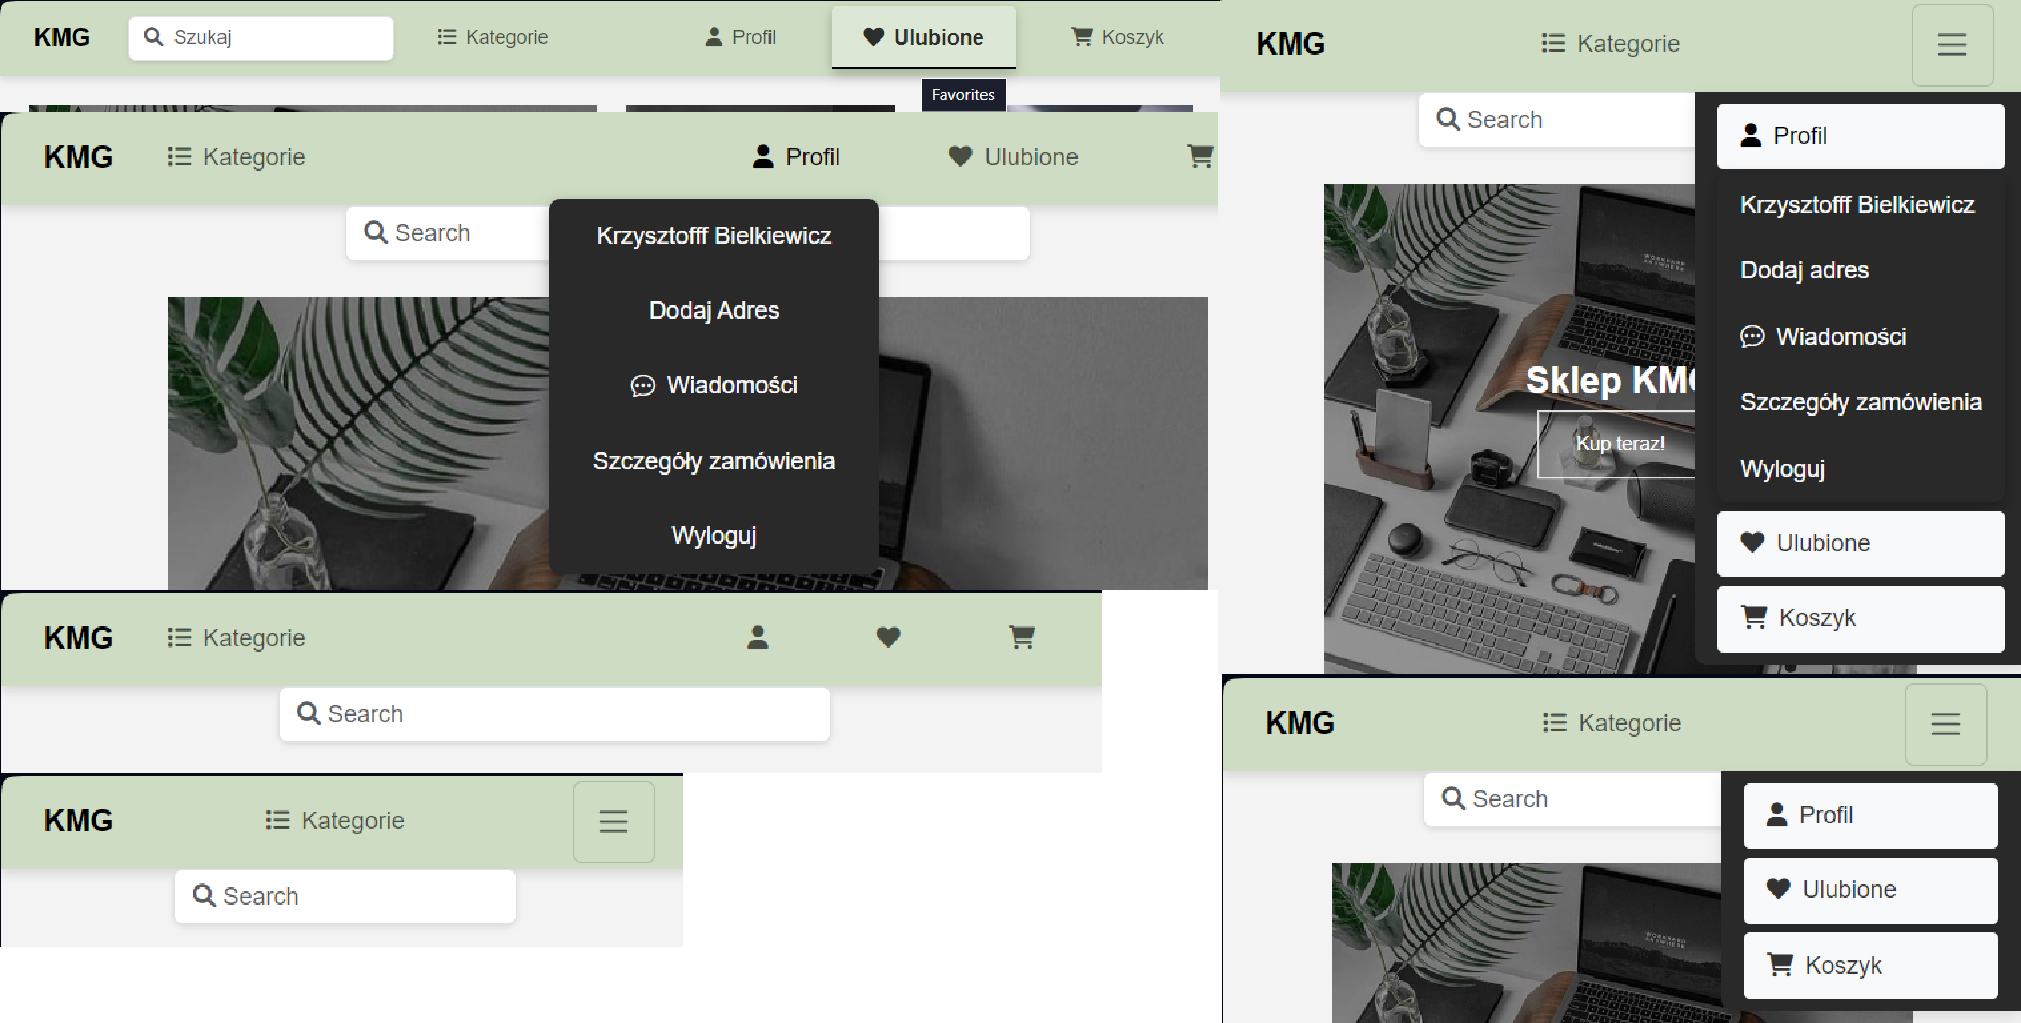
\includegraphics[width=0.9\columnwidth]{images/krzysztofBImages/header.png}
    \caption{Nagłówek z przyciskami}
\end{figure}

\begin{figure}[H]
    \centering
    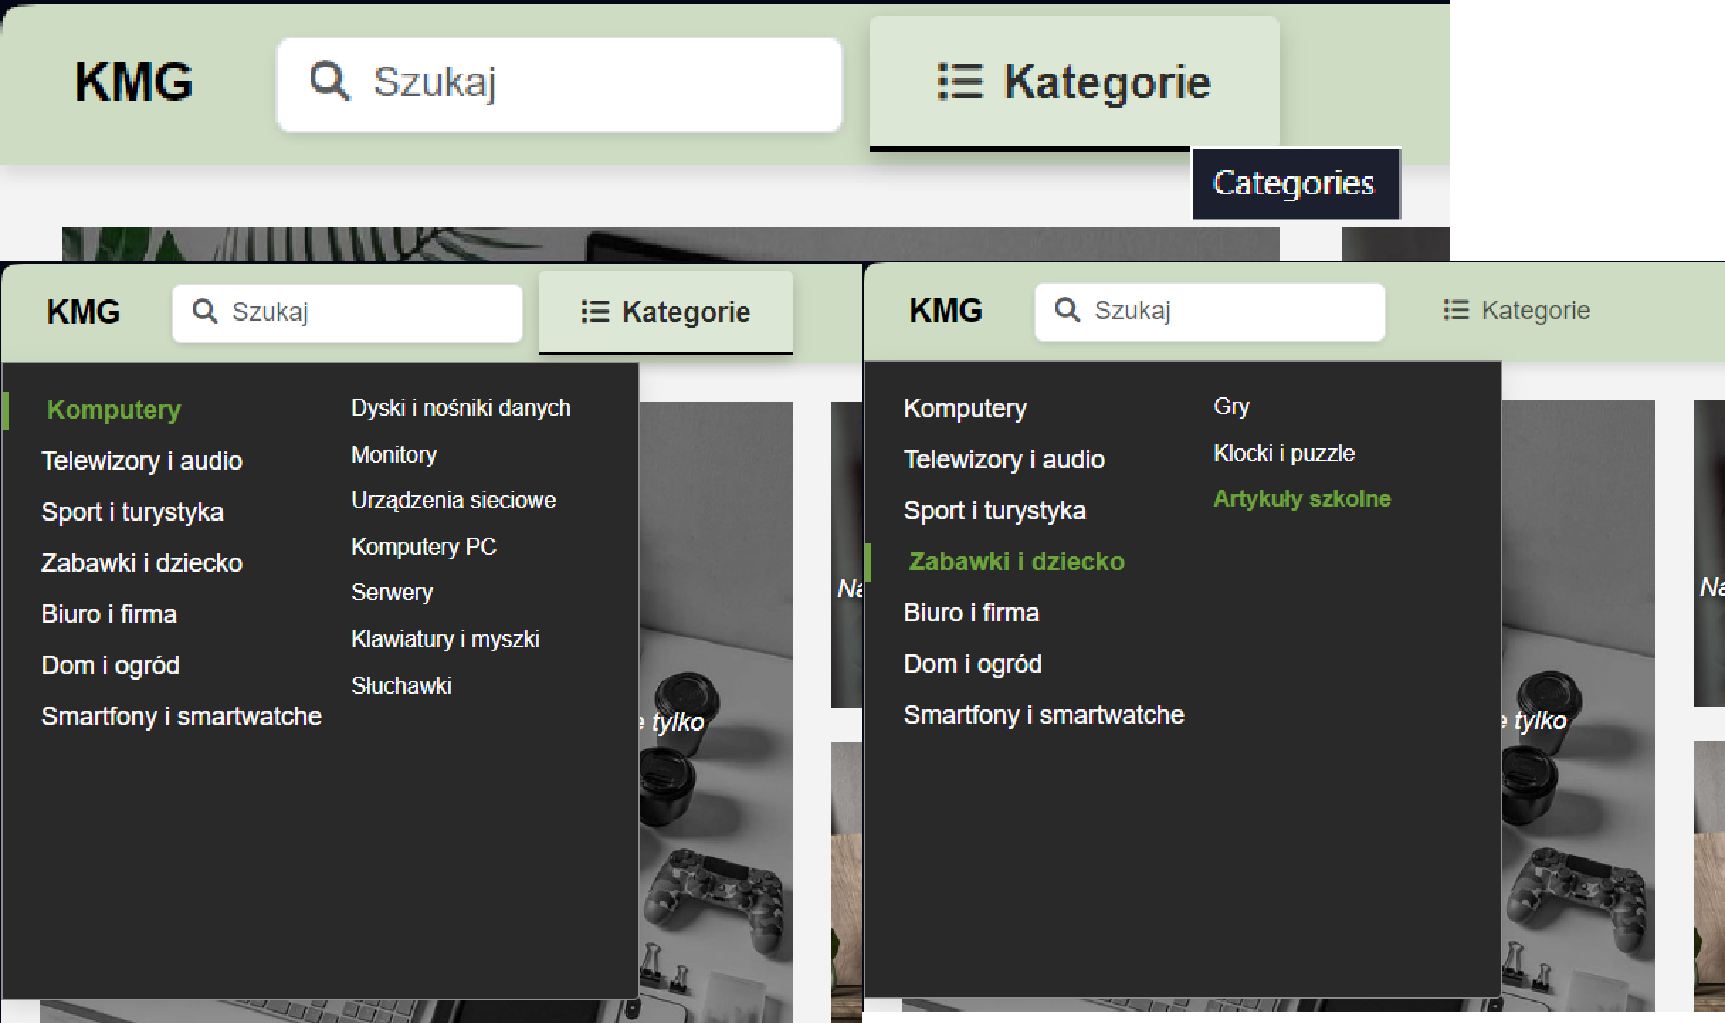
\includegraphics[width=0.9\columnwidth]{images/krzysztofBImages/header-categories.png}
    \caption{Wybór kategorii w nagłówku}
    \label{header-categories}
\end{figure}


\subsubsection{Krzysztof Bielkiewicz: Stworzenie strony startowej}
\label{1.3.2}
\textit{Responsywna strona startowa zawierająca:}
    \begin{itemize}
        \item Główny baner z przekierowaniami do poszczególnych kategorii
        \item Interaktywny slider wyświetlający polecane produkty oraz drugi co wyświetla polubione produkty
        \item Stopka
    \end{itemize}

    \begin{figure}[H]
        \centering
        
\includegraphics[width=0.8\columnwidth]{images/krzysztofBImages/main-banner.png}
        \caption{Główny banner}
    \end{figure}

    \begin{figure}[H]
        \centering
        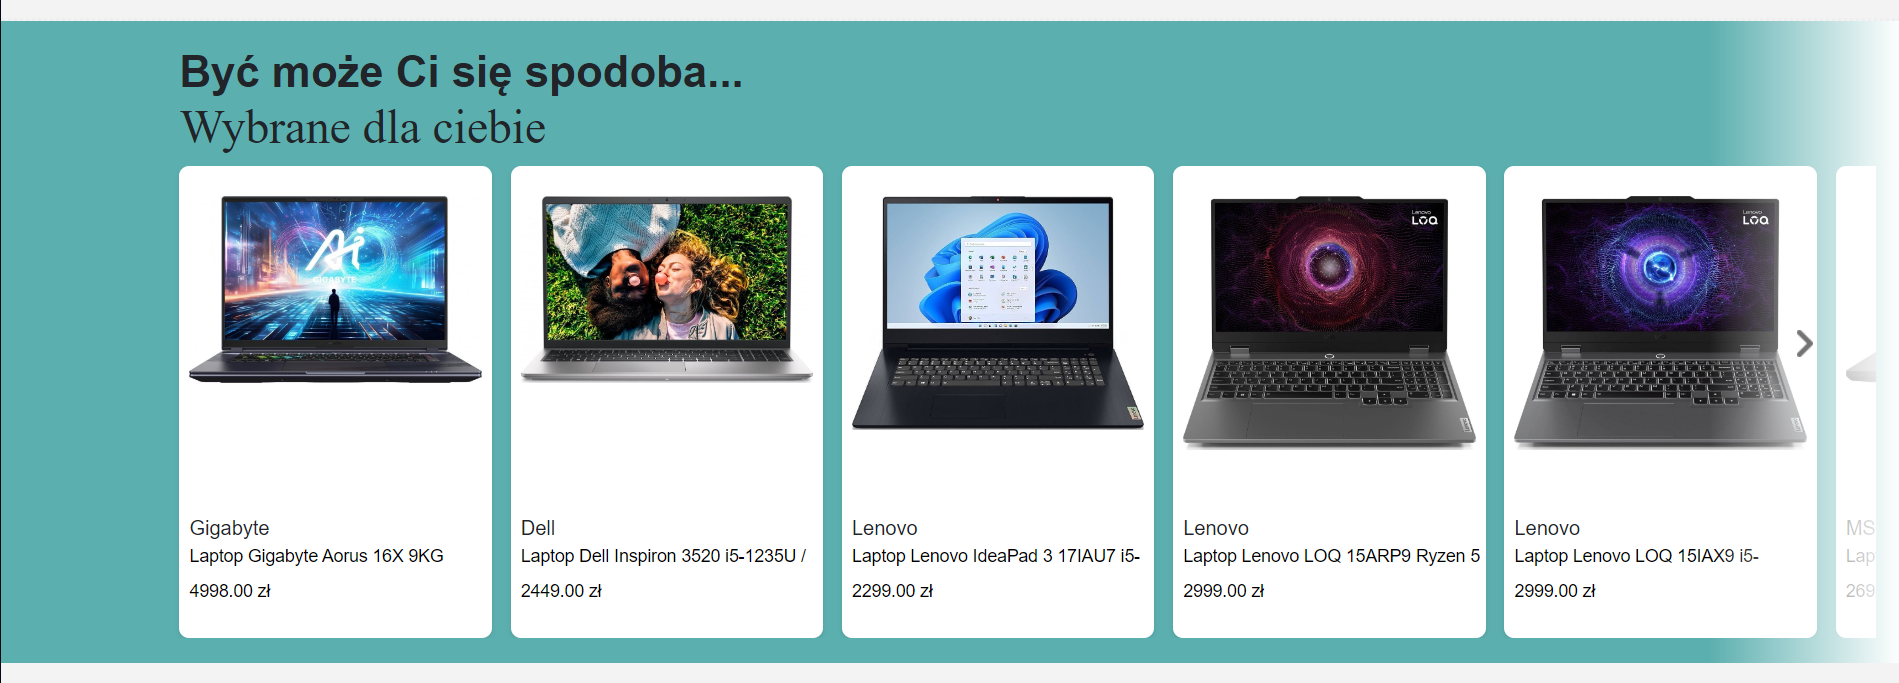
\includegraphics[width=0.7\columnwidth]{images/krzysztofBImages/slider-polecane.png}
        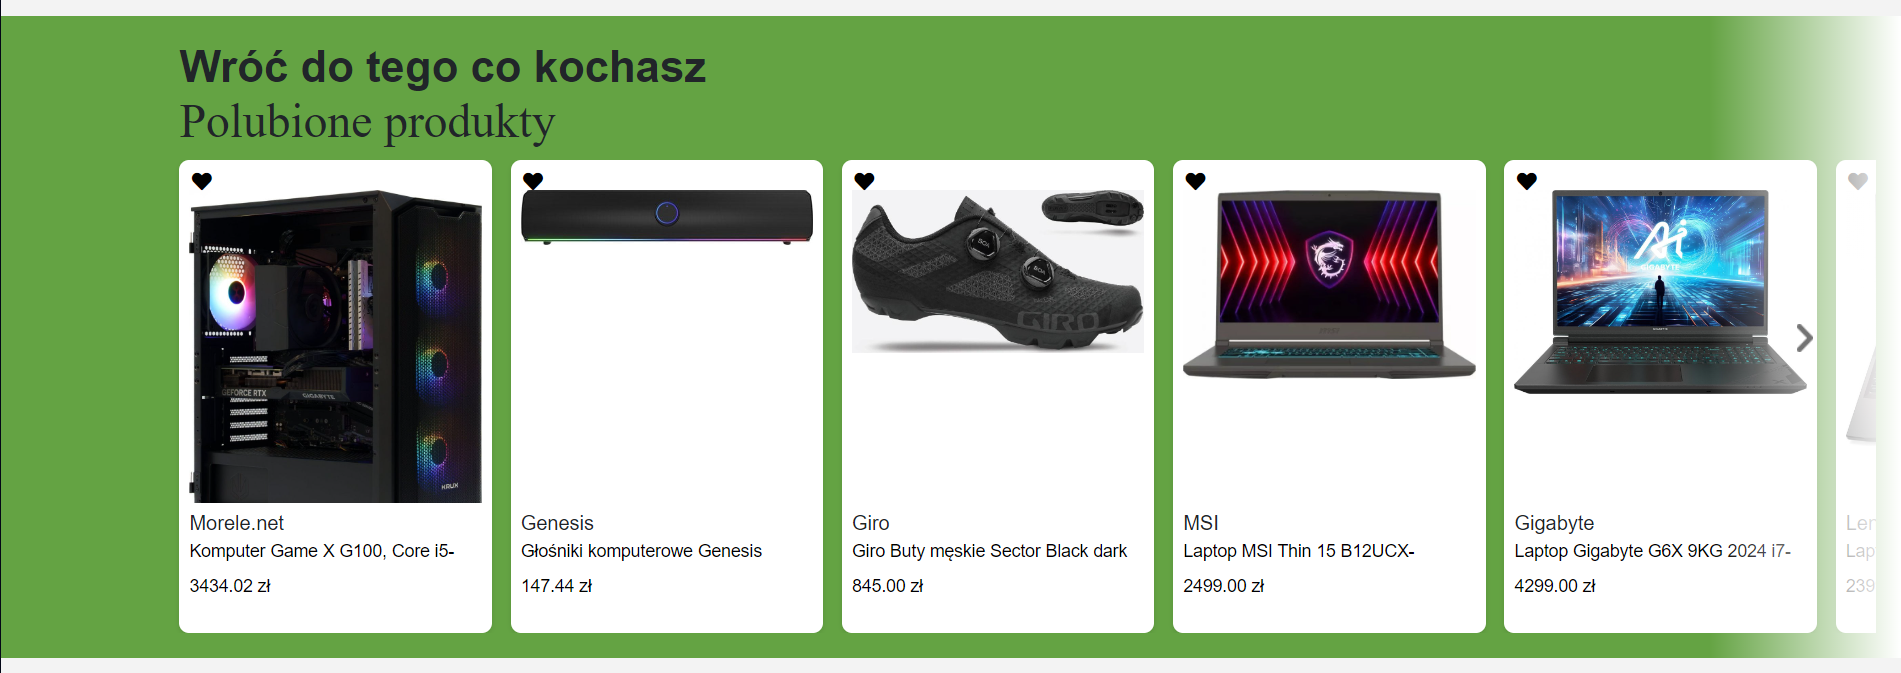
\includegraphics[width=0.7\columnwidth]{images/krzysztofBImages/slider-ulubione.png}
        \caption{Slider z polecanymi i polubionymi}
    \end{figure}

    \begin{figure}[H]
        \centering
        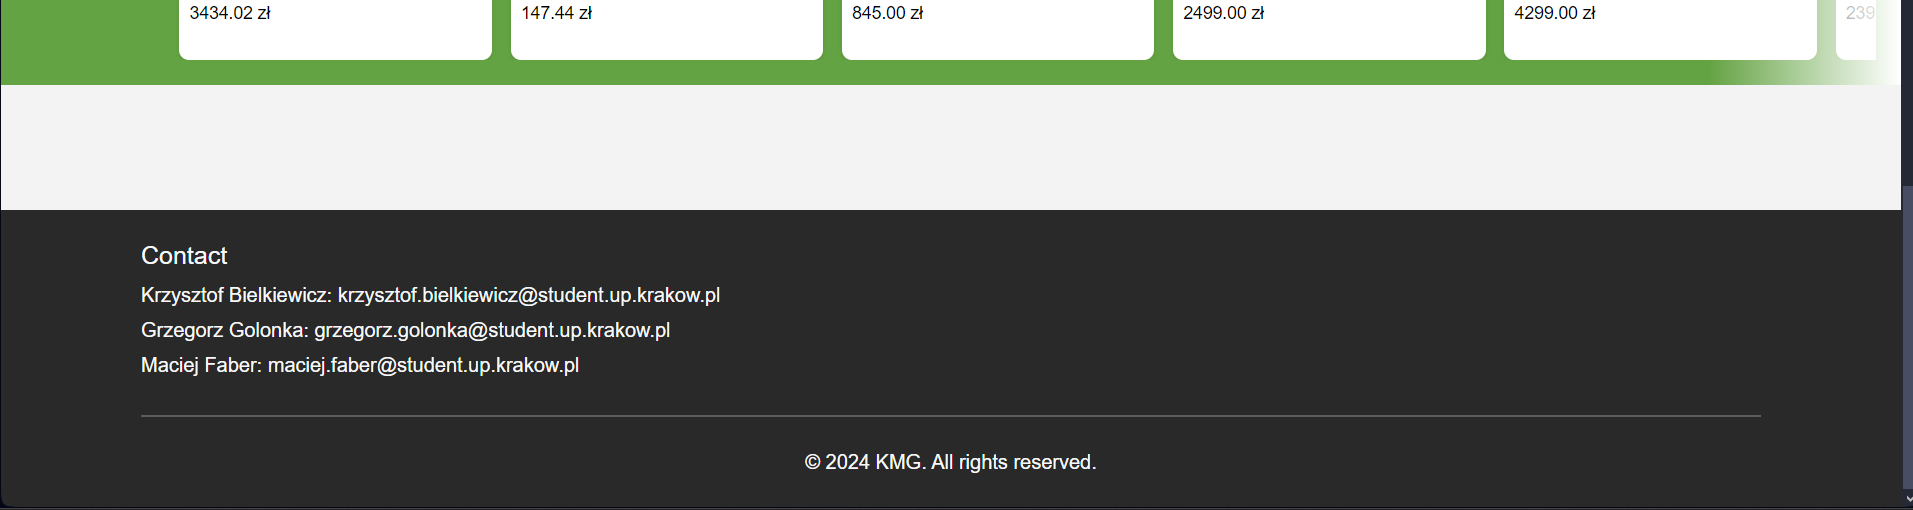
\includegraphics[width=0.7\columnwidth]{images/krzysztofBImages/footer.png}
        \caption{Stopka}
    \end{figure}


\subsubsection{Krzysztof Bielkiewicz: Opcja wyszukiwania po słowach kluczowych}
\label{1.3.3}
\textit{Implementacja w backend wyszukiwania po słowach wpisanych w rubryce 'Szukaj'
oraz strona wyświetlająca wynik wyszukiwania i jej oprawa graficzna.}
\begin{figure}[H]
    \centering
    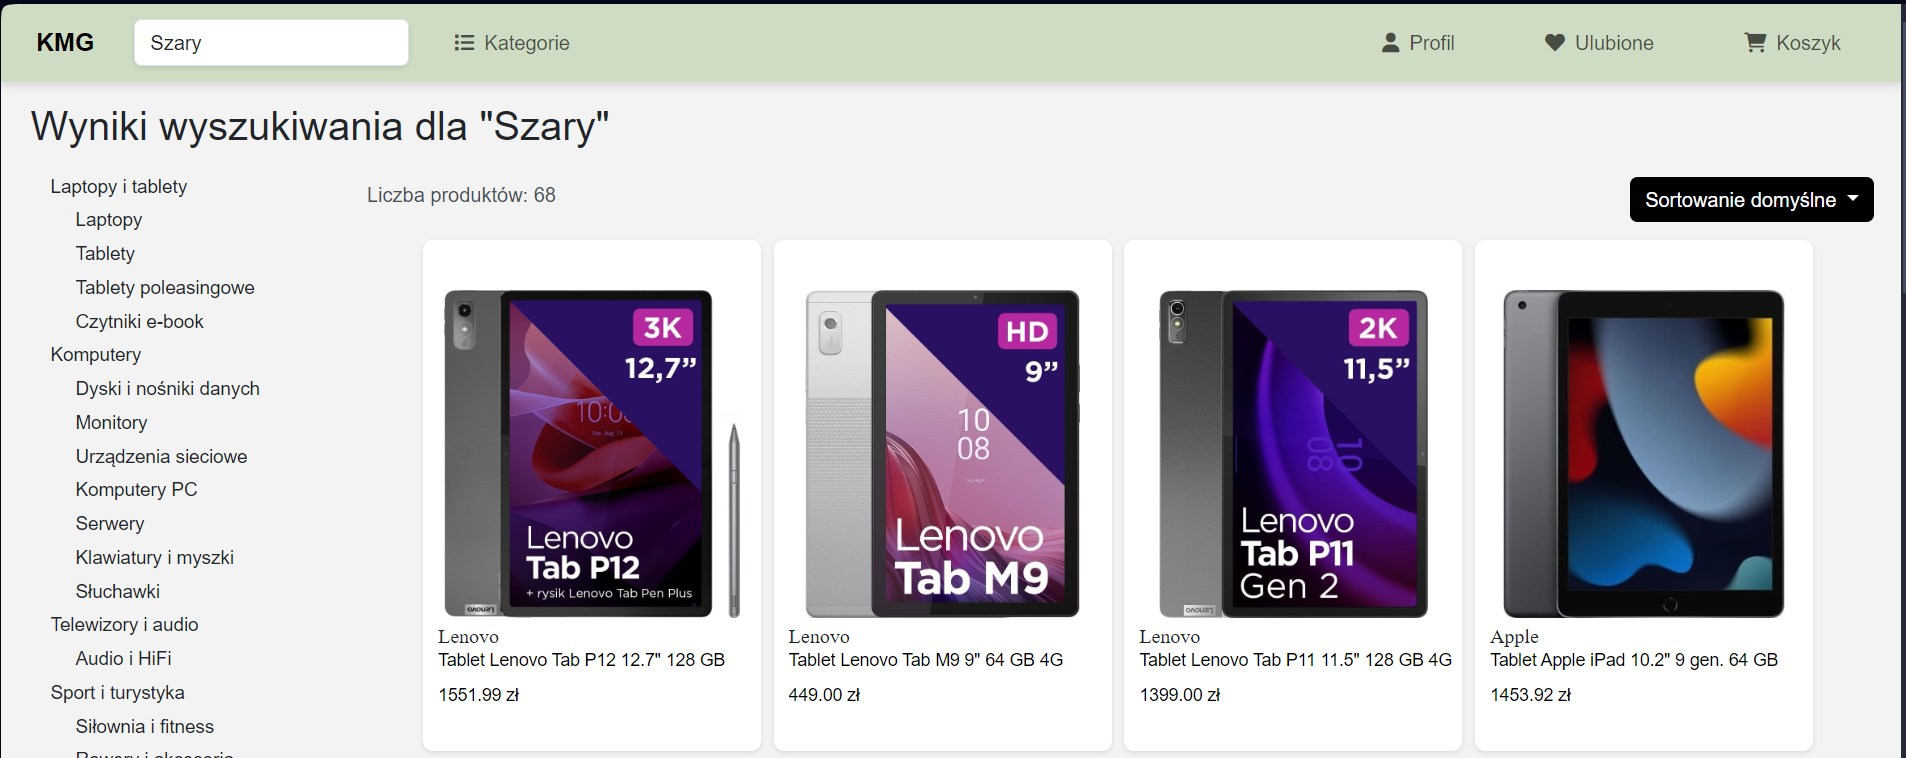
\includegraphics[width=0.8\columnwidth]{images/krzysztofBImages/wyszukiwanie.png}
    \caption{Wynik wyszukiwania}
\end{figure}

    
\subsubsection{Krzysztof Bielkiewicz: Opcja wyszukiwania po kategoriach}
\label{1.3.4}
    \textit{Zaimplementowana w backend opcja wyszukiwania po kategoriach
     oraz stworzenie w frontend liste kategorii w nagłówku
      oraz liste kategorii po lewej stronie od wyświetlanych produktów w której jest zaznaczona
      aktualnie przeglądana kategoria. Utworzenie strony z wyświetlanymi produktami z wybranej kategorii.}
    \begin{center}
        \hyperref[header-categories]{Zdjęcie wyszukiwania po kategoriach w nagłówku}
    \end{center}

    \begin{figure}[H]
        \centering
        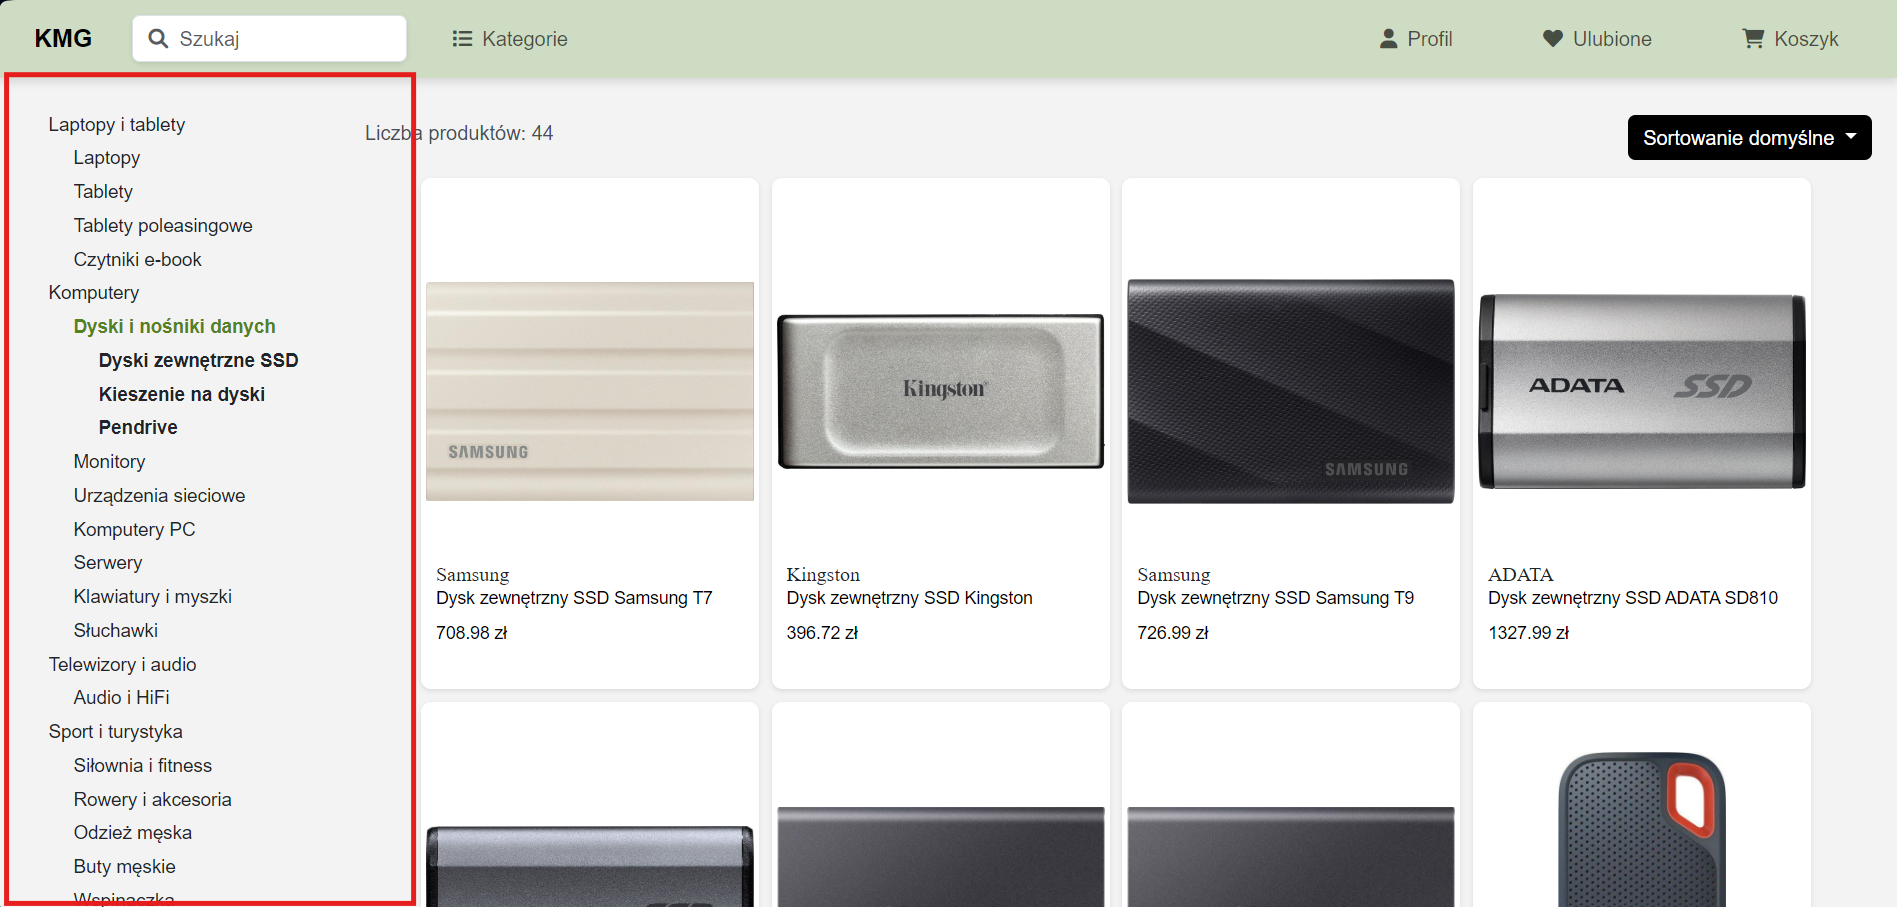
\includegraphics[width=0.8\columnwidth]{images/krzysztofBImages/lewe-kategorie.png}
        \caption{Kategorie po lewej stronie na stronie z produktami z wybranej kategorii}
    \end{figure}


\subsubsection{Krzysztof Bielkiewicz: Stworzenie strony z ulubionymi produktami}
\label{1.3.5}
\textit{Strona wyświetlająca produkty polubione przez użytkownika/lub w danej sesji.}

\begin{figure}[H]
    \centering
    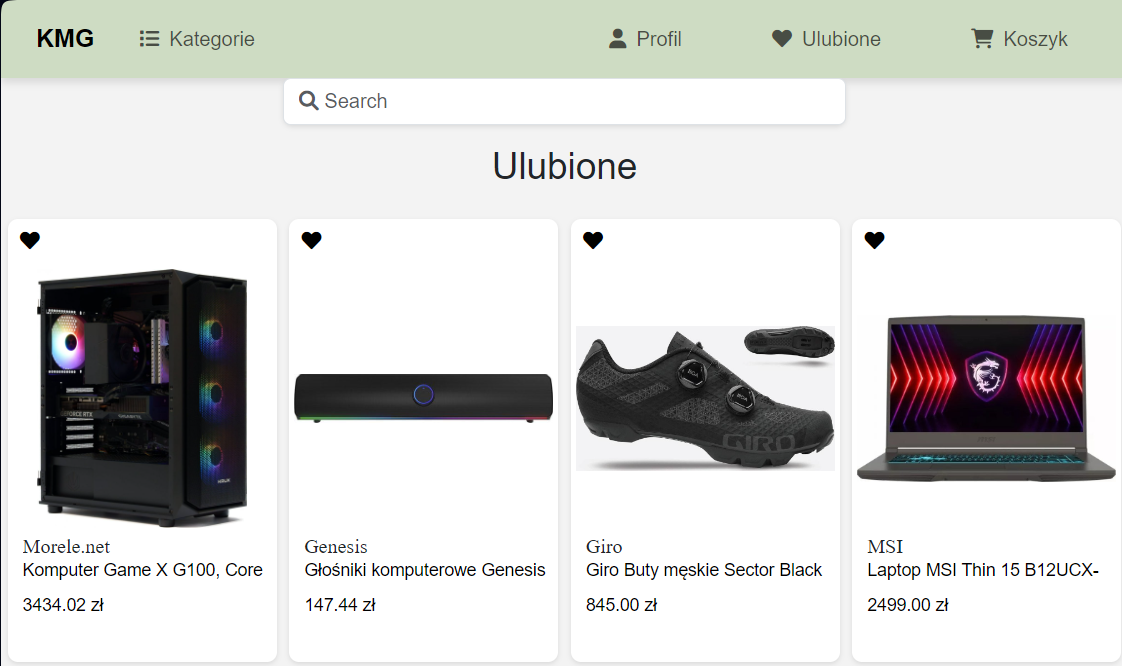
\includegraphics[width=0.8\columnwidth]{images/krzysztofBImages/strona-ulubione.png}
    \caption{Strona z polubionymi produktami}
\end{figure}

\subsubsection{Krzysztof Bielkiewicz: Stworzenie strony profilu z opcją edycji}
\label{1.3.6}
\textit{Stworzenie responsywnej strony w backend i frontend do edycji danych z modelu User.
Umożliwia edycje podstawych danych jak e-mail, imię, date urodzenia, itp.
Oraz umożliwia zmianę hasła.}

\begin{figure}[H]
    \centering
    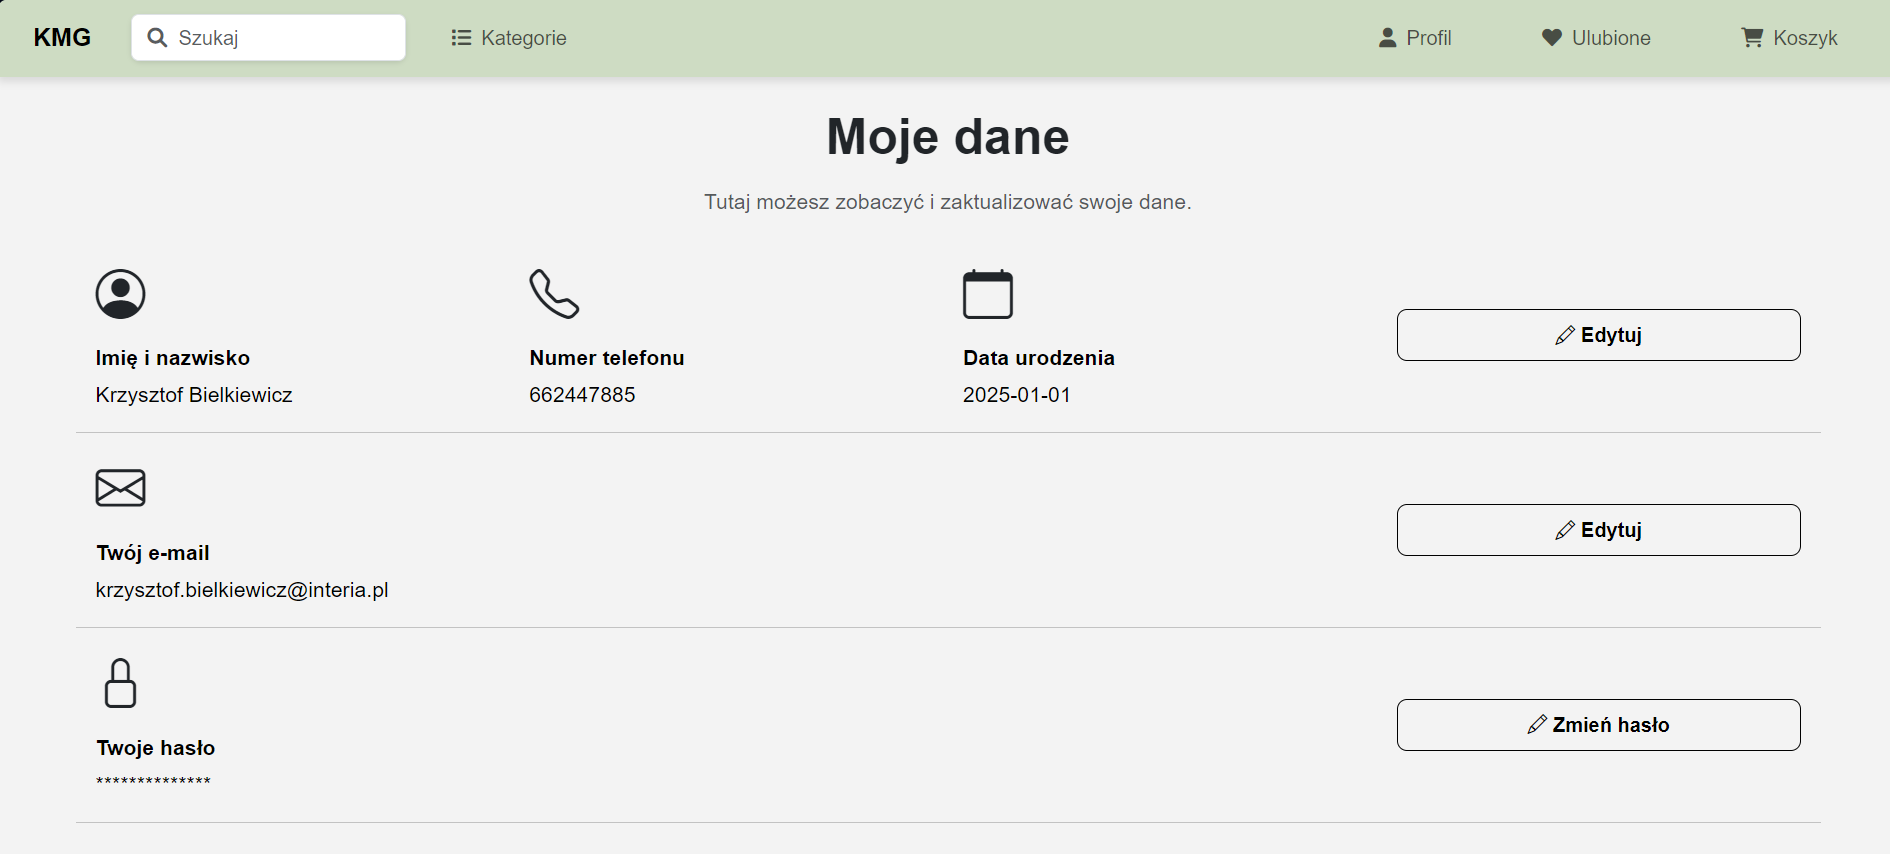
\includegraphics[width=0.9\columnwidth]{images/krzysztofBImages/profil/strona-edycji-profilu.png}
    \caption{Strona z polami do edycji profilu}
\end{figure}

\begin{figure}[H]
    \centering
    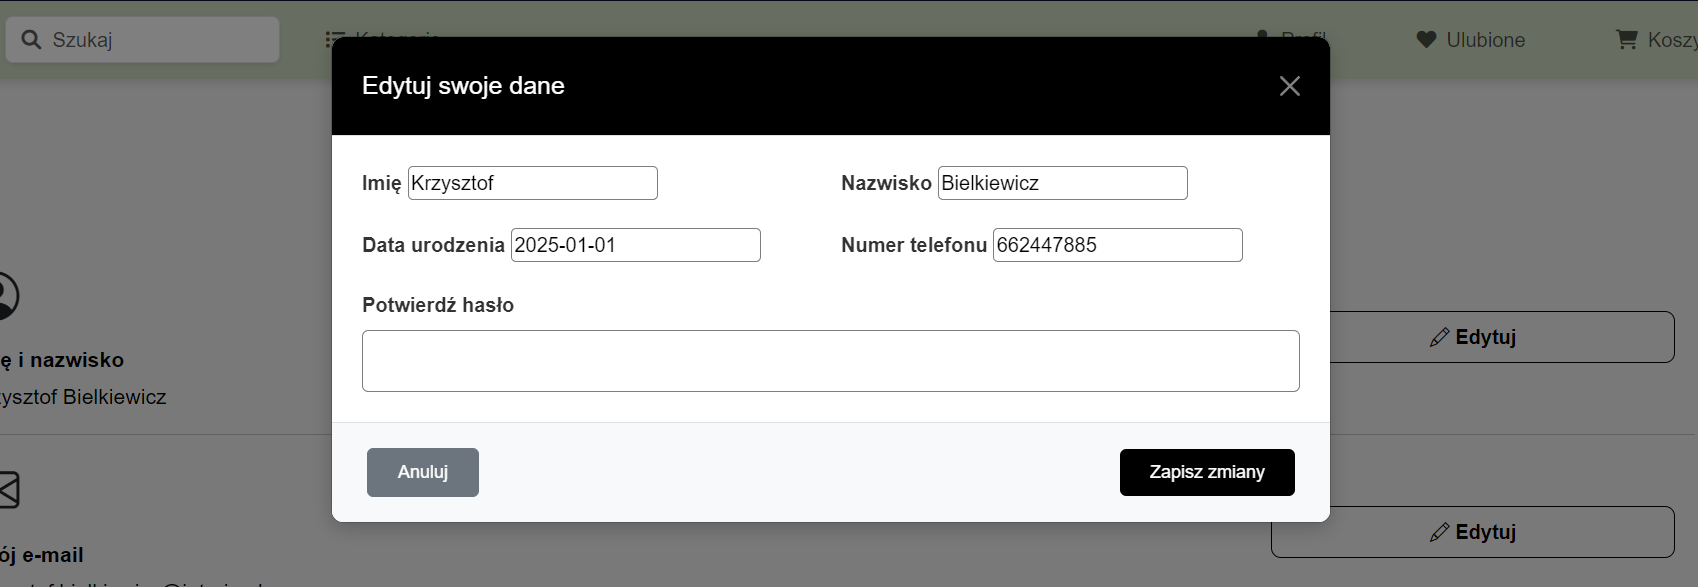
\includegraphics[width=0.9\columnwidth]{images/krzysztofBImages/profil/edycja-danych.png}
    \caption{Formularz edytowania podstawowych danych}
\end{figure}

\begin{figure}[H]
    \centering
    \includegraphics[width=0.9\columnwidth]{images/krzysztofBImages/profil/zmiana-hasła.png}
    \caption{Formularz zmiany hasła}
\end{figure}

\begin{figure}[H]
    \centering
    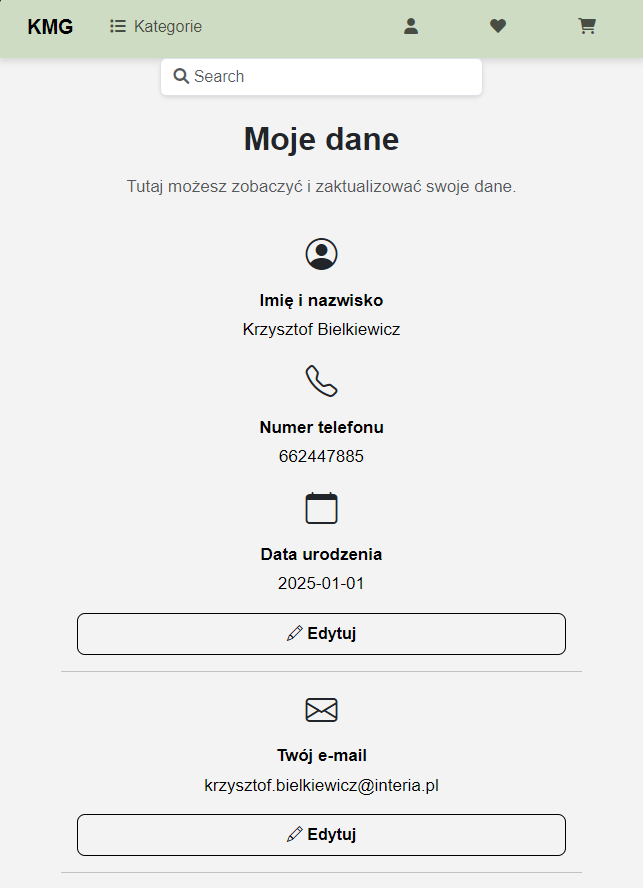
\includegraphics[width=0.5\columnwidth]{images/krzysztofBImages/profil/responywna-strona-profilu.png}
    \caption{Responywna strona edycji profilu}
\end{figure}

\subsubsection{Krzysztof Bielkiewicz: Oprawa graficzna strony adresu dostawy}
\label{1.3.7}
\textit{Utworzenie oprawy graficznej dla strony dodania adresu dostawy.}
\begin{figure}[H]
    \centering
    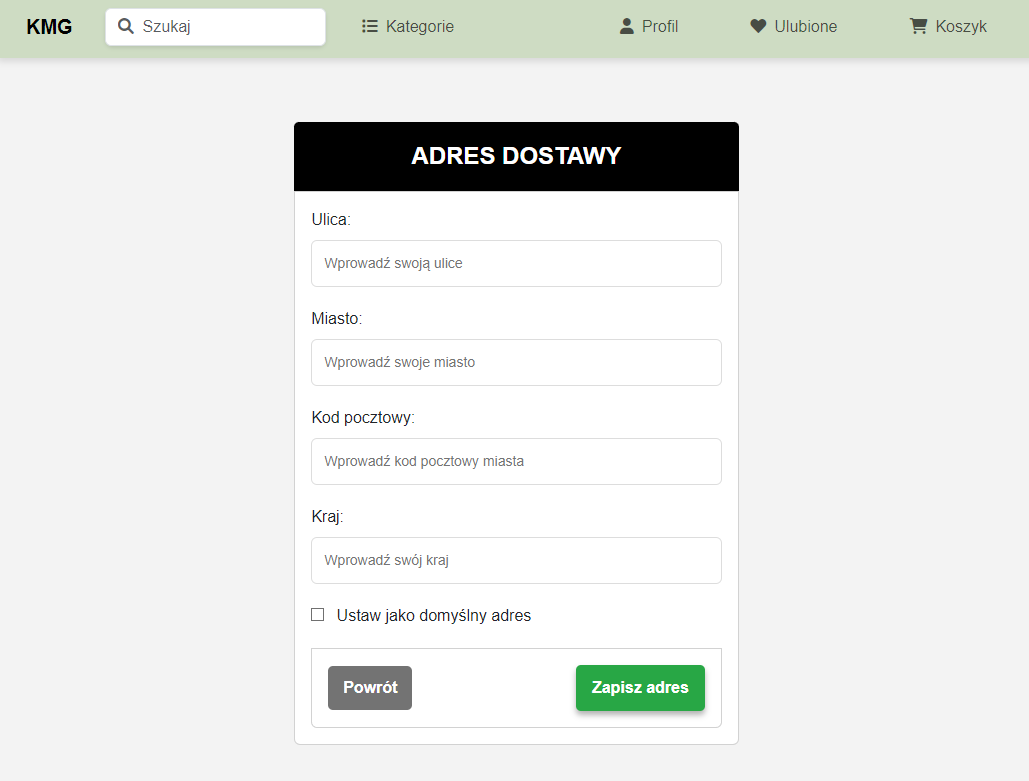
\includegraphics[width=0.8\columnwidth]{images/krzysztofBImages/strona-dodaj-adres.png}
    \caption{Strona z formularzem dodania adresu dostawy}
\end{figure}

\subsubsection{Krzysztof Bielkiewicz: Oprawa graficzna koszyka}
\label{1.3.8}
\textit{Utworzenie oprawy graficznej dla koszyka i jej responywność.}
\begin{figure}[H]
    \centering
    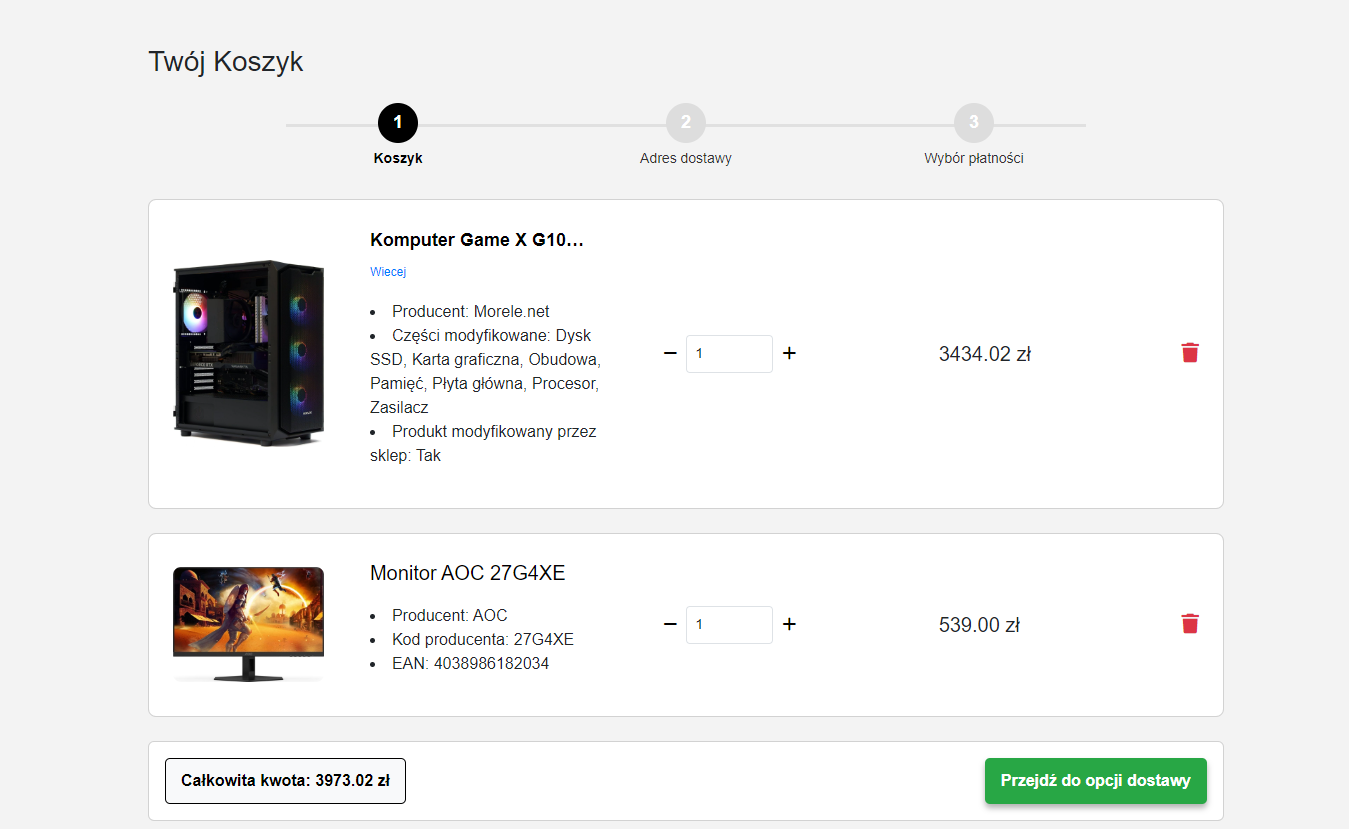
\includegraphics[width=0.8\columnwidth]{images/krzysztofBImages/cart/cart-step1.png}
    \caption{Strona koszyka}
\end{figure}

\begin{figure}[H]
    \centering
    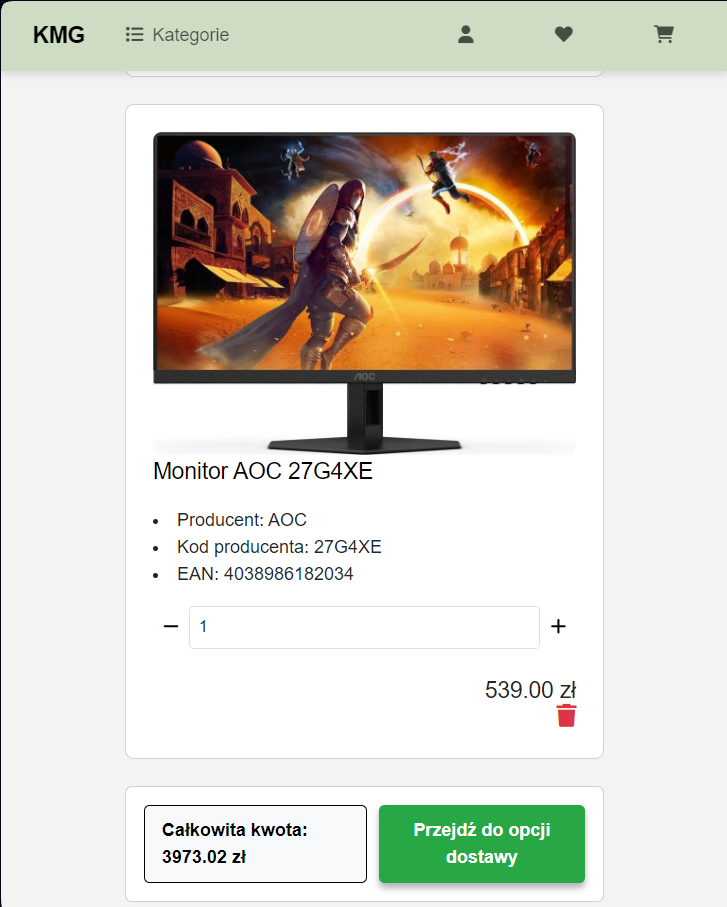
\includegraphics[width=0.5\columnwidth]{images/krzysztofBImages/cart/cart-step1-respo.png}
    \caption{Strona koszyka - responsywna}
\end{figure}

\subsubsection{Krzysztof Bielkiewicz: Oprawa graficzna wyboru adresu dostawy}
\label{1.3.9}
\textit{Utworzenie oprawy graficznej dla wyboru adresu dostawy.}
\begin{figure}[H]
    \centering
    \includegraphics[width=0.8\columnwidth]{images/krzysztofBImages/cart/wybór-adresu-dostawy.png}
    \caption{Strona wyboru adresu dostawy}
\end{figure}

\subsubsection{Krzysztof Bielkiewicz: Oprawa graficzna dla metod płatności}
\label{1.3.10}
\textit{Utworzenie oprawy graficznej metod płatności.}
\begin{figure}[H]
    \centering
    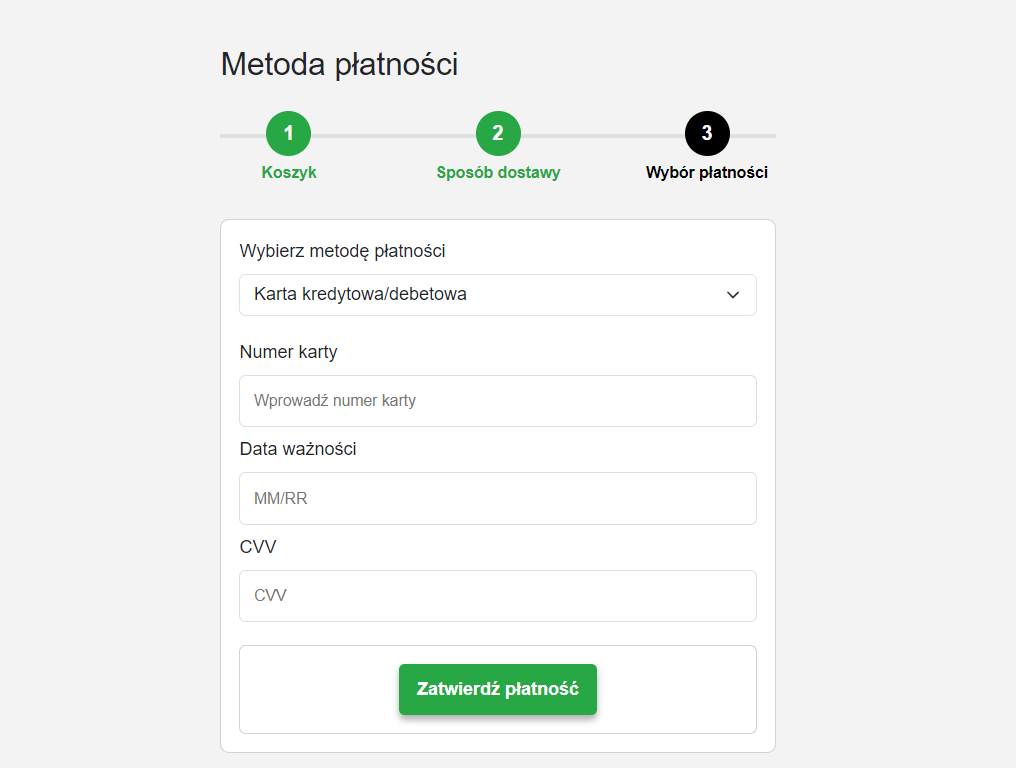
\includegraphics[width=0.8\columnwidth]{images/krzysztofBImages/cart/metody-płatności-karta.png}
    \caption{Metoda płatności kartą}
\end{figure}

\begin{figure}[H]
    \centering
    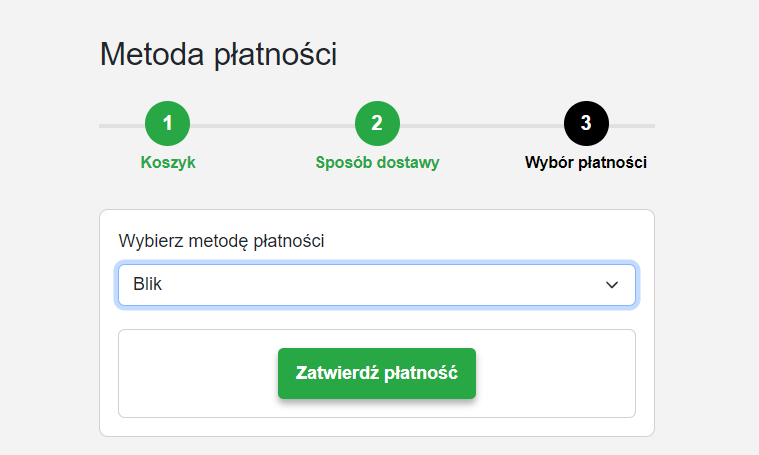
\includegraphics[width=1.0\columnwidth]{images/krzysztofBImages/cart/metody-płatności-blik.png}
    \caption{Metoda płatności blik}
\end{figure}

\begin{figure}[H]
    \centering
    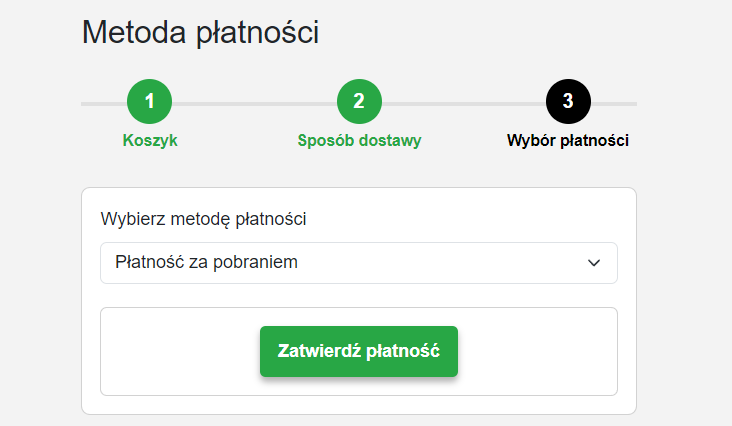
\includegraphics[width=0.8\columnwidth]{images/krzysztofBImages/cart/metody-płatności-za-pobraniem.png}
    \caption{Metoda płatności za pobraniem}
\end{figure}

\subsubsection{Krzysztof Bielkiewicz: Oprawa graficzna szczegółów zamówienia}
\label{1.3.11}
\textit{Utworzenie oprawy graficznej dla strony ze szegółami zamówienia i jej responywność.}

\begin{figure}[H]
    \centering
    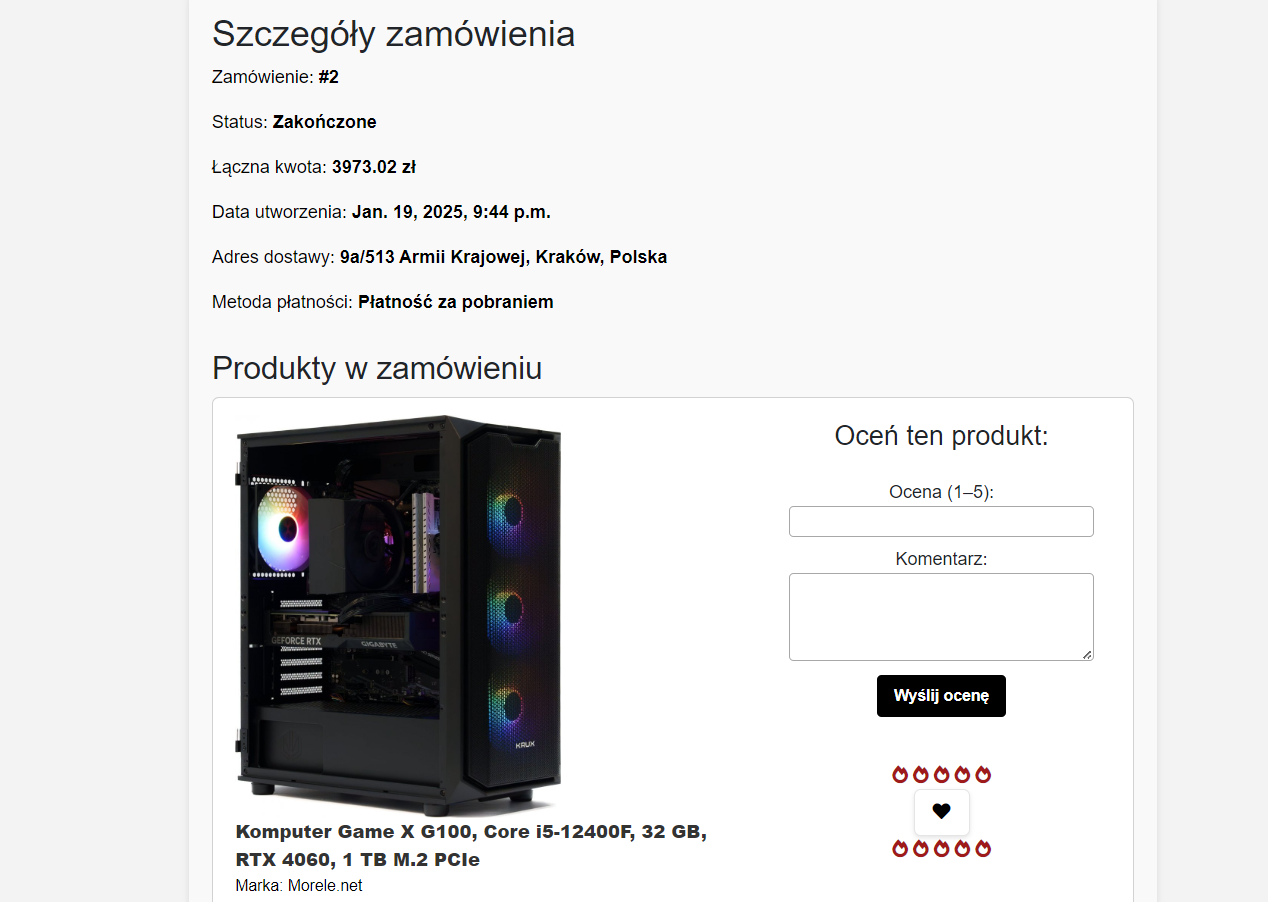
\includegraphics[width=0.8\columnwidth]{images/krzysztofBImages/szczegóły-zamówieniaV1.png}
    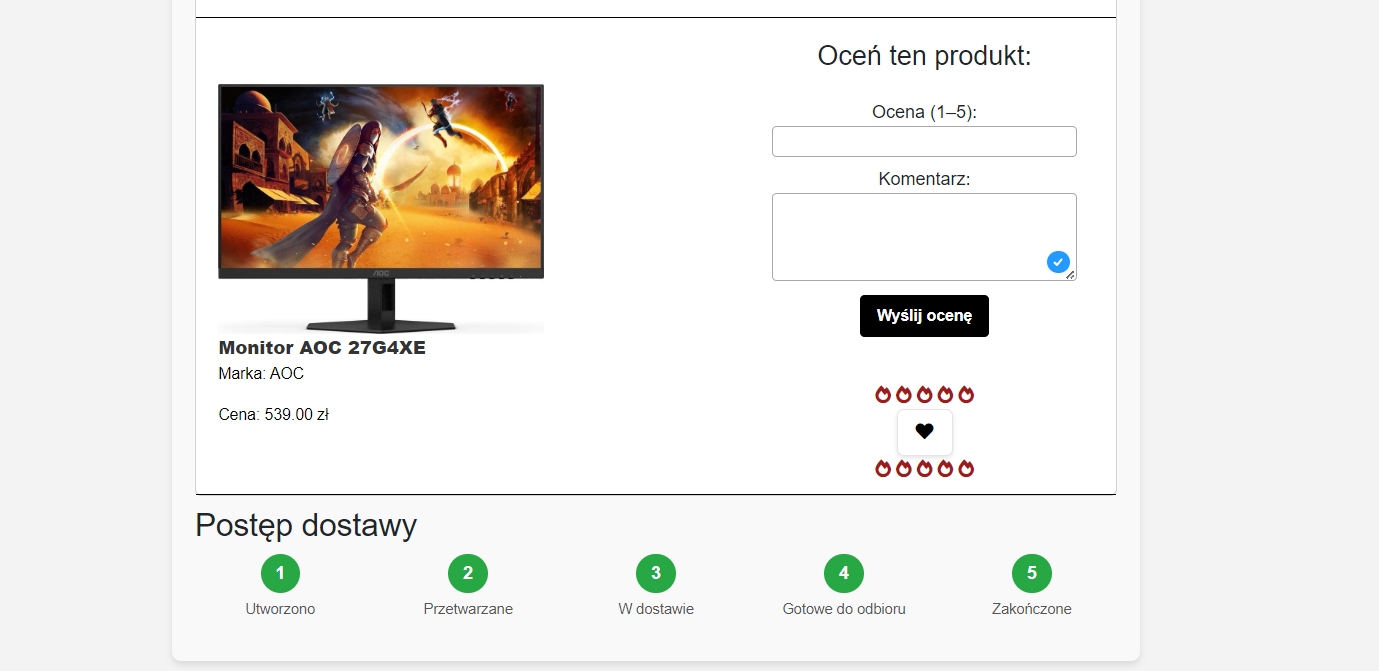
\includegraphics[width=0.8\columnwidth]{images/krzysztofBImages/szczegóły-zamówieniaV2.png}
    \caption{Strona ze szegółami zamówienia}
\end{figure}

\begin{figure}[H]
    \centering
    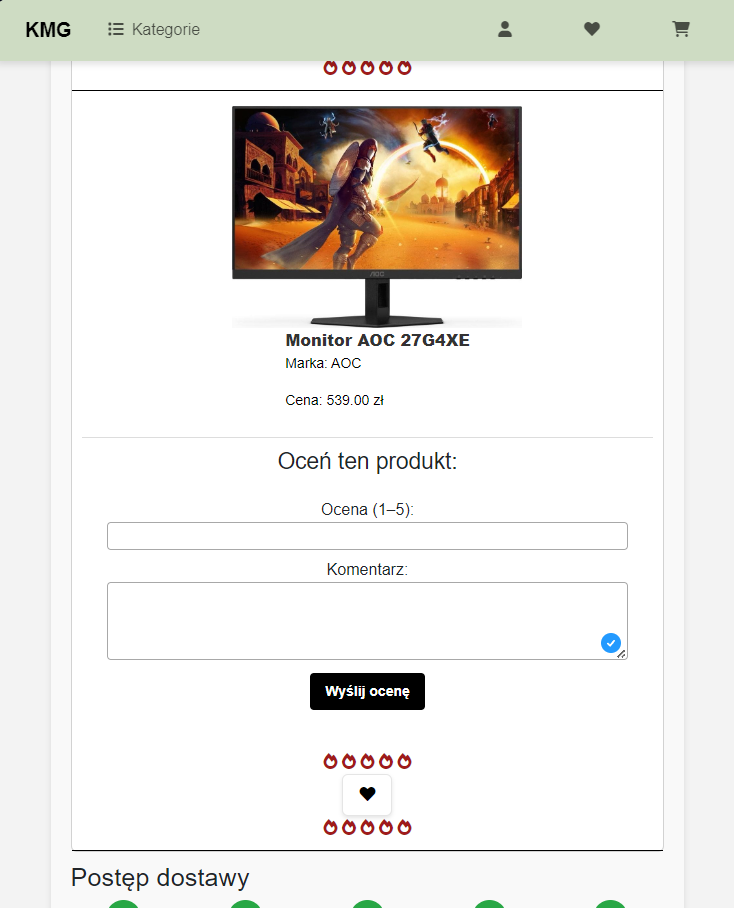
\includegraphics[width=0.5\columnwidth]{images/krzysztofBImages/szczegóły-zamówienia-respo.png}
    \caption{Responywna strona ze szegółami zamówienia}
\end{figure}

\subsubsection{Krzysztof Bielkiewicz: Oprawa graficzna dla listy zamówień}
\label{1.3.12}
\textit{Utworzenie oprawy graficznej dla listy zamówień.}

\begin{figure}[H]
    \centering
    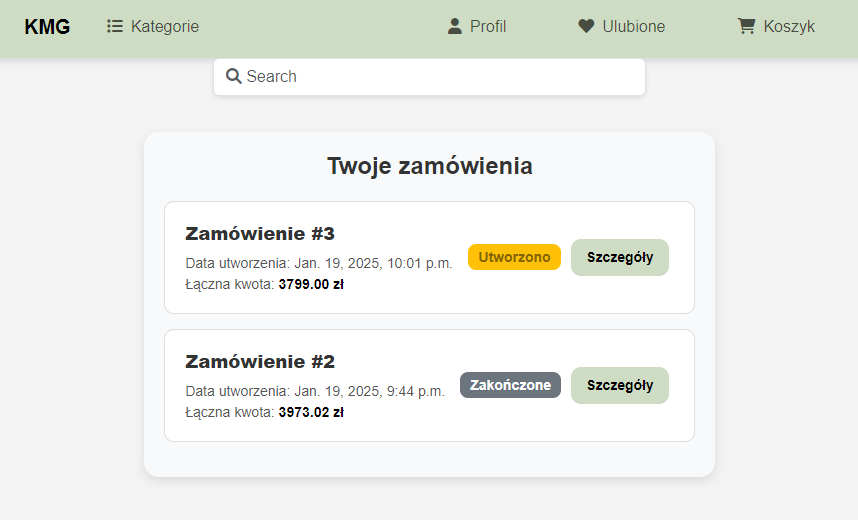
\includegraphics[width=0.8\columnwidth]{images/krzysztofBImages/orders.png}
    \caption{Lista zamówień}
\end{figure}


\subsubsection{Krzysztof Bielkiewicz: Wyświetlenie produktów z bazy danych}
\label{1.3.13}
\textit{Utworzenie strony wyświetlającej produkty z podstawowymi danymi: marka, tytuł, cena oraz zdjęcie.
Przyciski polubienia i koszyka dla każdego produktu po najechaniu na dany produkt.
Produkty polubione przez użytkownika mają widoczne serca.
Oprawa graficzna dla wyświetlanych prduktów i przycisków polubienia i dodania do koszyka.}
\begin{figure}[H]
    \centering
    \includegraphics[width=0.9\columnwidth]{images/krzysztofBImages/lista-produktów.png}
    \caption{Wyświetlanie listy produktów}
\end{figure}

\begin{figure}[H]
    \centering
    
\includegraphics[width=0.5\columnwidth]{images/krzysztofBImages/przyciski-polubienia-koszyka.png}
    \caption{Przyciski polubienia i dodania do koszyka.}
\end{figure}

\begin{figure}[H]
    \centering
    \includegraphics[width=0.5\columnwidth]{images/krzysztofBImages/lista-produktów-respo.png}
    \caption{Wyświetlanie listy produktów - responywność}
\end{figure}



\subsubsection{Krzysztof Bielkiewicz: Funkcja dodawania produktów do ulubionych}
\label{1.3.14}
\textit{Dodawanie produktów do ulubionych i usuwanie ich z ulubionych przy użyciu django.
Produkt po kliknięciu na przycisk sreca dodaje się do Ulubionych i za poconą skrytu 
JavaScript zmienia ikonke serca na czarne wypełnione. Dane produkty pojawiają się na stronie Ulubione.
Po kliknięciu z powrotem na wypełnione serce produkt usuwa się ulubionych.
Produkty polubione zapisują się w danej sesji i po zalogowaniu są wysyłane do polubień danego usera,
co zapewnia wygode dla użytkownika.}


\subsubsection{Krzysztof Bielkiewicz: Paginacja produktów na stronach}
\label{1.3.15}
\textit{Paginacja dla stron 'Wszystkie produkty', 'Produkty z kategorii', 'Wyszukane produkty', 'Ulubione'.}
\begin{figure}[H]
    \centering
    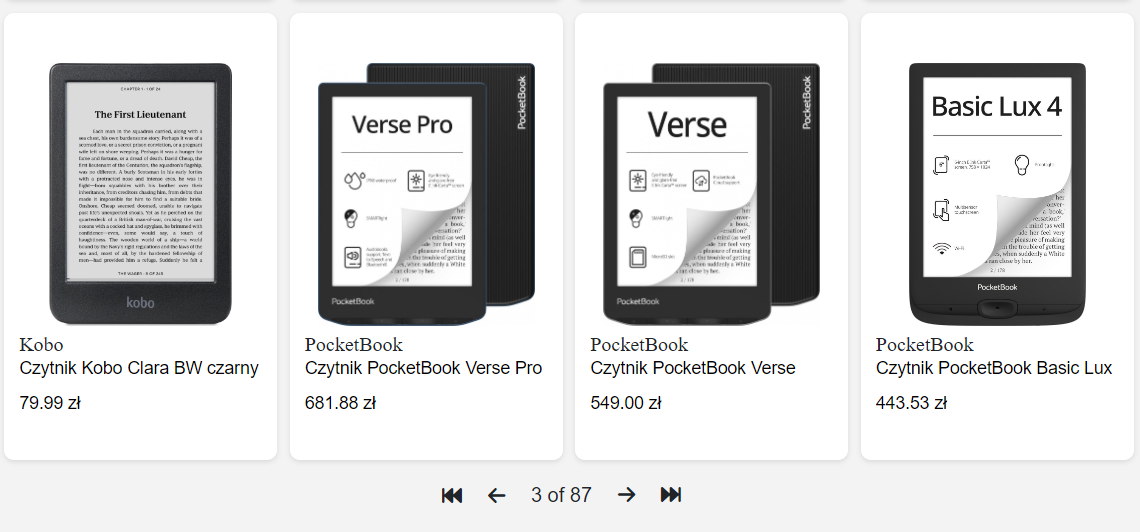
\includegraphics[width=1.0\columnwidth]{images/krzysztofBImages/pagination.png}
    \caption{Paginacja}
\end{figure}


\subsubsection{Krzysztof Bielkiewicz: Oprawa graficzna szczegółów produktu}
\label{1.3.16}
\textit{Oprawa graficzna dla szegółów produktu i jej responywność.}
\begin{figure}[H]
    \centering
    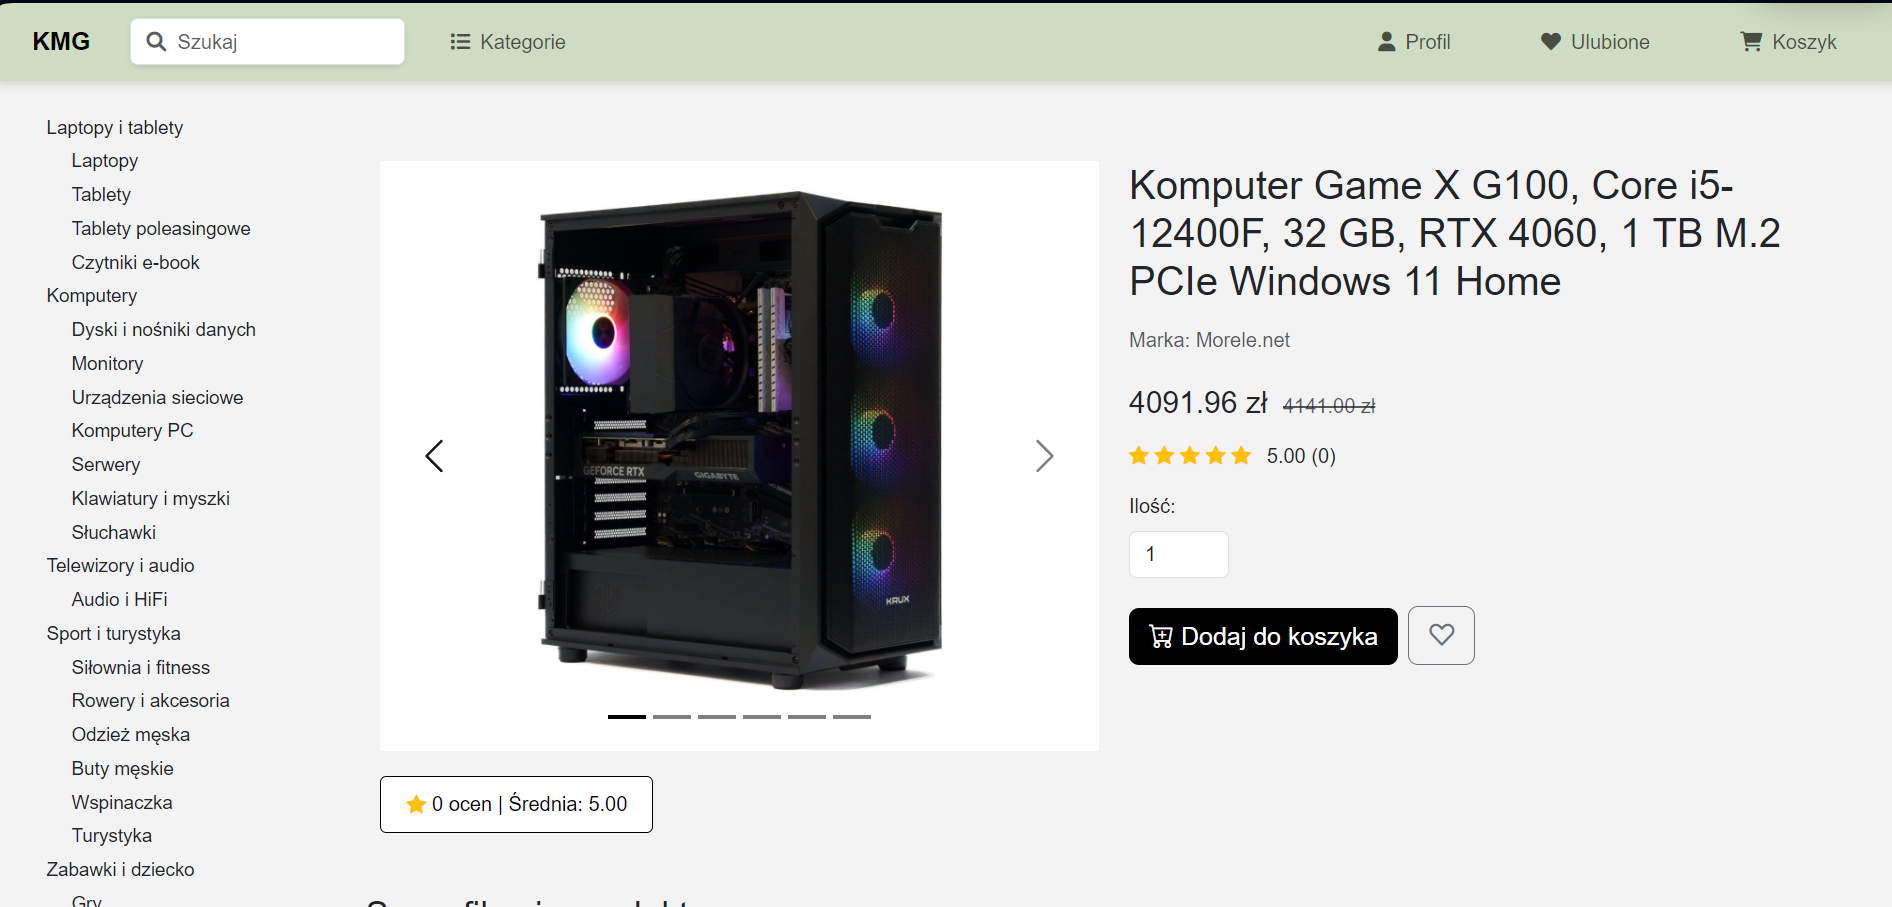
\includegraphics[width=1.0\columnwidth]{images/krzysztofBImages/product-detail.png}
    \caption{Szczegóły produkt}
\end{figure}
\begin{figure}[H]
    \centering
    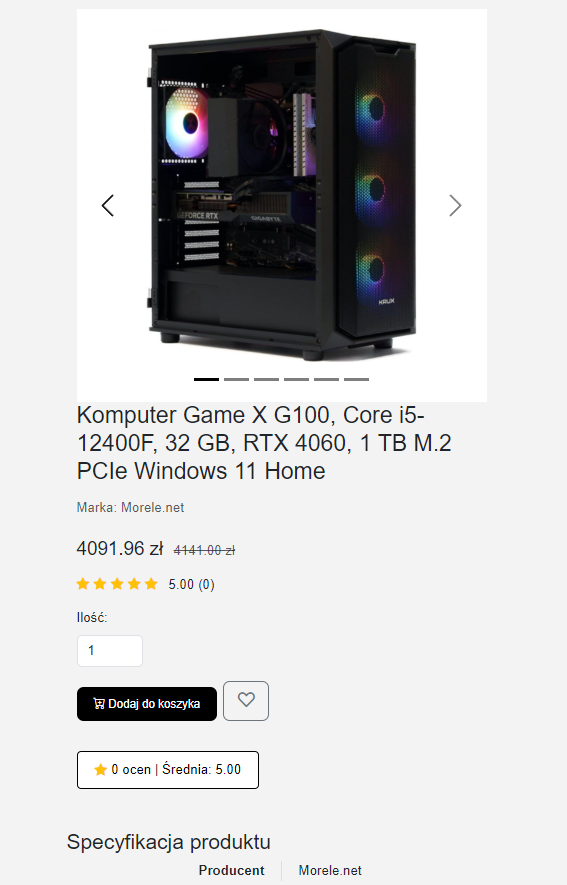
\includegraphics[width=0.5\columnwidth]{images/krzysztofBImages/product-detail-respo.png}
    \caption{Szczegóły produkt - responywna wersja}
\end{figure}

\subsubsection{Krzysztof Bielkiewicz: Custom errory i oprawa graficzna rejestracji}
\label{1.3.17}
\textit{Własne errory wyświetlające się pod wymaganymi polami,
pole telefonu z automatycznym formatem zrobionym w JS,
 wybór daty urodzenia z zablokowanym wyborem daty w przyszłości (JS). Oprawa graficzna.
 Oraz okienko powiadamiające o udanej rejestracji.}

\begin{figure}[H]
    \centering
    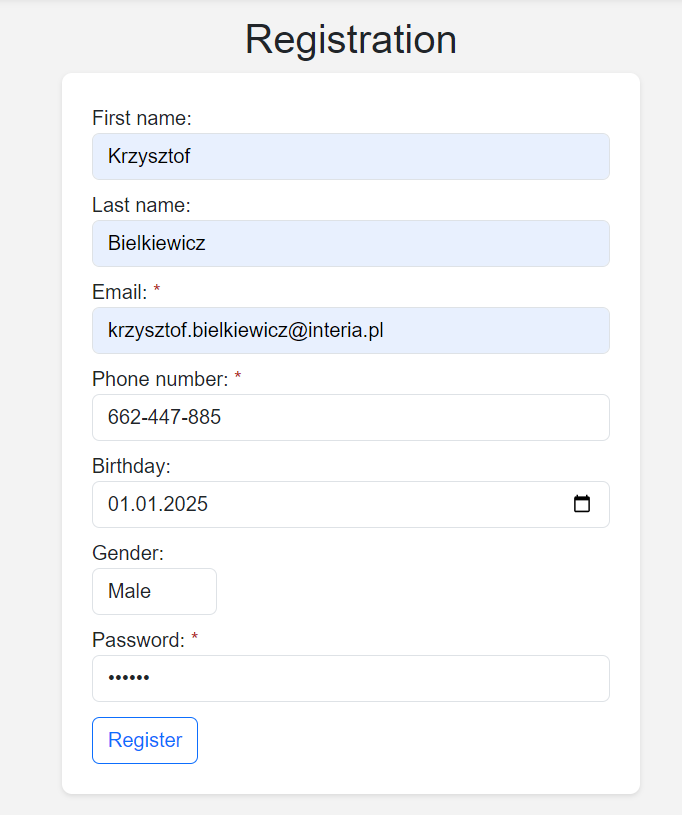
\includegraphics[width=0.5\columnwidth]{images/krzysztofBImages/register-login/registration.png}
    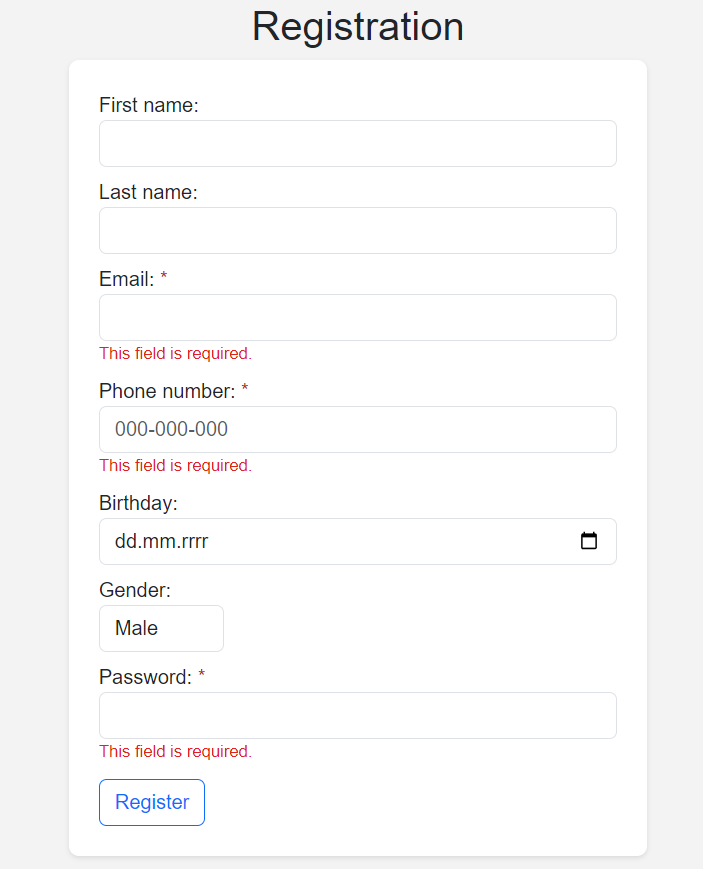
\includegraphics[width=0.48\columnwidth]{images/krzysztofBImages/register-login/register-errors.png}
    \caption{Rejestracja}
    \label{register}
\end{figure}
\begin{figure}[H]
    \centering
    
\includegraphics[width=0.6\columnwidth]{images/krzysztofBImages/register-login/message.png}
    \caption{Powiadomienie}
    \label{message}
\end{figure}


\subsubsection{Krzysztof Bielkiewicz: Custom errory i oprawa graficzna loginu}
\label{1.3.18}
\textit{Oprawa graficzna. Własne errory wyświetlające się pod wymaganymi polami.}

\begin{figure}[H]
    \centering
    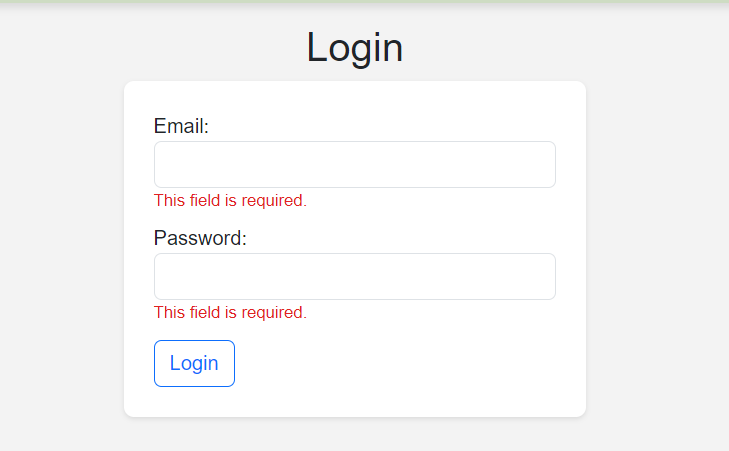
\includegraphics[width=0.8\columnwidth]{images/krzysztofBImages/register-login/login.png}
    \caption{Login}
    \label{login}
\end{figure}



%  Zadania Grzegorz Golonka
\subsubsection{Grzegorz Golonka: Utworzenie pliku README.md }
\label{section:1.3.19}
\textit{Przygotowanie szczegółowego pliku README.md dla projektu \texttt{kmg\_store},
 zawierającego opis projektu, spis treści, funkcjonalności,
 modele bazodanowe oraz instrukcję instalacji i użycia aplikacji.
Plik README.md został stworzony w sposób przejrzysty i intuicyjny,
co ułatwia zrozumienie struktury projektu oraz jego uruchomienie przez nowych użytkowników i deweloperów.}
\begin{figure}[H]
    \centering
    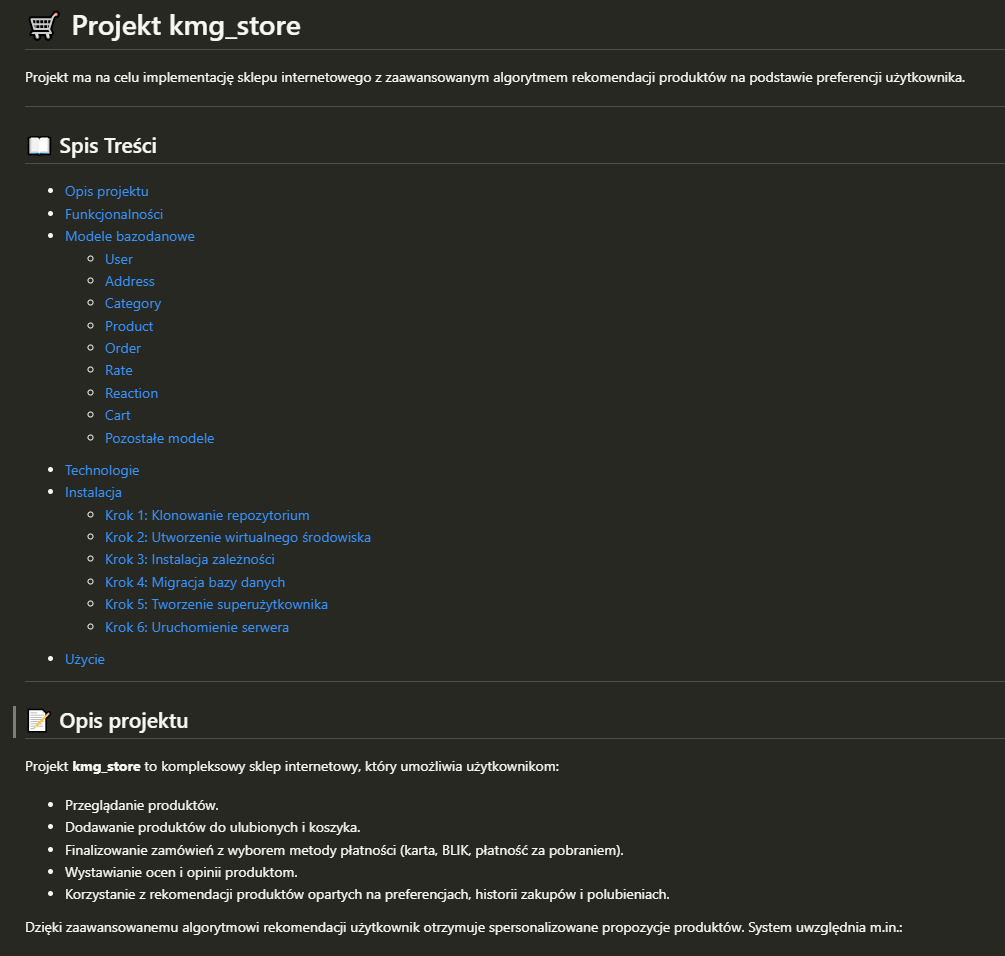
\includegraphics[width=0.9\columnwidth]{images/krzysztofBImages/readme_preview.png}
    \caption{Widok pliku README.md dla projektu \textbf{kmg\_store}}
\end{figure}
%
%
\subsubsection{Grzegorz Golonka: Utworzenie modeli bazodanowych}
\label{section:1.3.20}
Przygotowanie głównych modeli bazodanowych dla projektu \texttt{kmg\_store}.
W ramach tego zadania zaimplementowano struktury danych w pliku \texttt{models.py},
obejmujące m.in. modele użytkowników (\texttt{User}), adresów dostawy (\texttt{Address}),
metod płatności (\texttt{PaymentMethod}), kategorii produktów (\texttt{Category}),
zamówień (\texttt{Order}), produktów (\texttt{Product}) oraz dodatkowe modele wspierające
takie jak reakcje użytkowników (\texttt{Reaction}) czy modele (\texttt{Conversation}).

Modele zostały zaprojektowane zgodnie z wymaganiami projektu, uwzględniając relacje między tabelami,
walidację danych oraz dodatkowe funkcje wspierające, takie jak obliczanie średniej oceny produktu,
zarządzanie ulubionymi produktami czy obsługa historii interakcji użytkownika.
Dzięki temu stworzono elastyczną i wydajną strukturę bazy danych,
umożliwiającą rozwój funkcjonalności sklepu internetowego w przyszłości.

\begin{figure}[H]
    \centering
    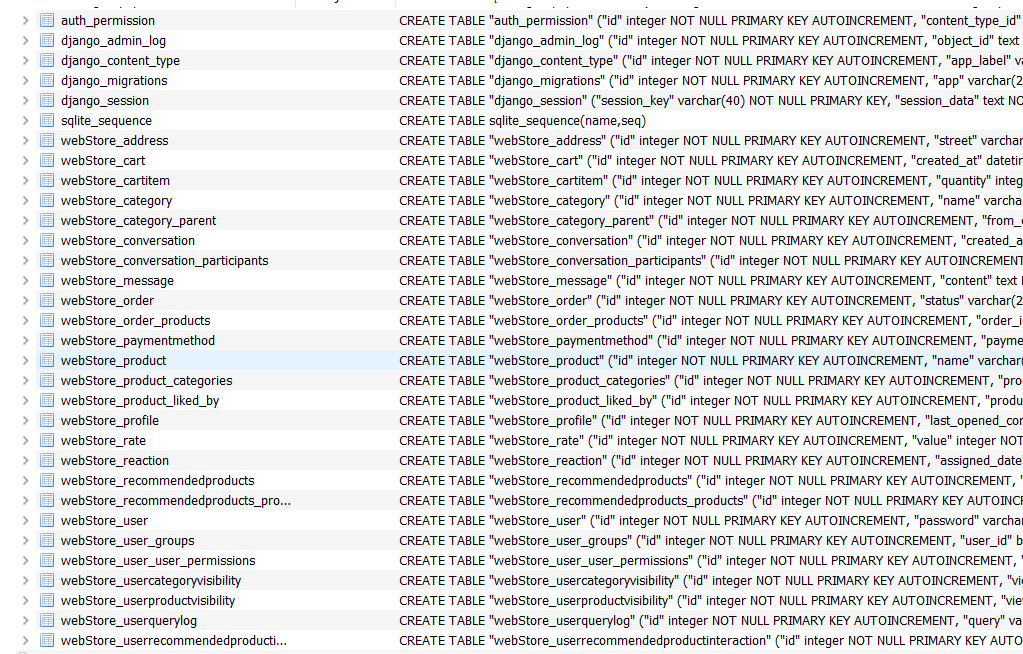
\includegraphics[width=0.9\columnwidth]{images/krzysztofBImages/modele_bazodanowe.png}
    \caption{Widok tabel w przeglądarce DB Browser for SQLite}
    \label{fig:db_models}
\end{figure}


%
%
\subsubsection{Grzegorz Golonka: Dodanie skryptów do inicjalizacji projektu}
\label{section:1.3.21}
Dodanie skryptów wspierających inicjalizację projektu \texttt{kmg\_store}. W ramach tego zadania przygotowano dwa główne skrypty:

\begin{itemize}
    \item \texttt{create\_superuser.py} – Skrypt umożliwiający automatyczne tworzenie konta superużytkownika. Skrypt weryfikuje, czy konto z określonym loginem już istnieje, a jeśli nie, tworzy je z domyślnymi danymi.
    \item \texttt{init\_project\_bash.sh} – Skrypt powłokowy automatyzujący proces inicjalizacji środowiska projektu. Obejmuje m.in. tworzenie i aktywację wirtualnego środowiska, instalację zależności, zarządzanie migracjami oraz uruchamianie serwera Django.
    \item \texttt{init\_project\_shell.ps} – Adekwatny skrypt do \texttt{init\_project\_bash.sh}, ale w wersji shellowej.
\end{itemize}

Skrypty te znacząco upraszczają proces przygotowania środowiska programistycznego, co przyczynia się do większej efektywności pracy zespołu.


Skrypty te znacząco upraszczają proces przygotowania środowiska programistycznego, co przyczynia się do większej efektywności pracy zespołu.
%
%
\subsubsection{Grzegorz Golonka: Stworzenie seeda produktów i kategorii}
\label{section:1.3.22}
\textit{
Przygotowanie skryptów do generowania danych testowych produktów i kategorii. Skrypty automatycznie pobierają dane z analizy znaczników HTML stron internetowych i zapisują je w formacie JSON. Zrealizowane zadania obejmują:
}
\begin{itemize}
    \item Pobieranie linków do produktów i tworzenie struktur kategorii.
    \item Zapisywanie szczegółowych danych produktów, takich jak nazwa, cena, zdjęcia i specyfikacje.
    \item Grupowanie i filtrowanie linków według wzorców.
\end{itemize}

\textit{
Skrypty te znacząco ułatwiają przygotowanie danych do testowania i wdrażania aplikacji.
}

\begin{figure}[H]
    \centering
    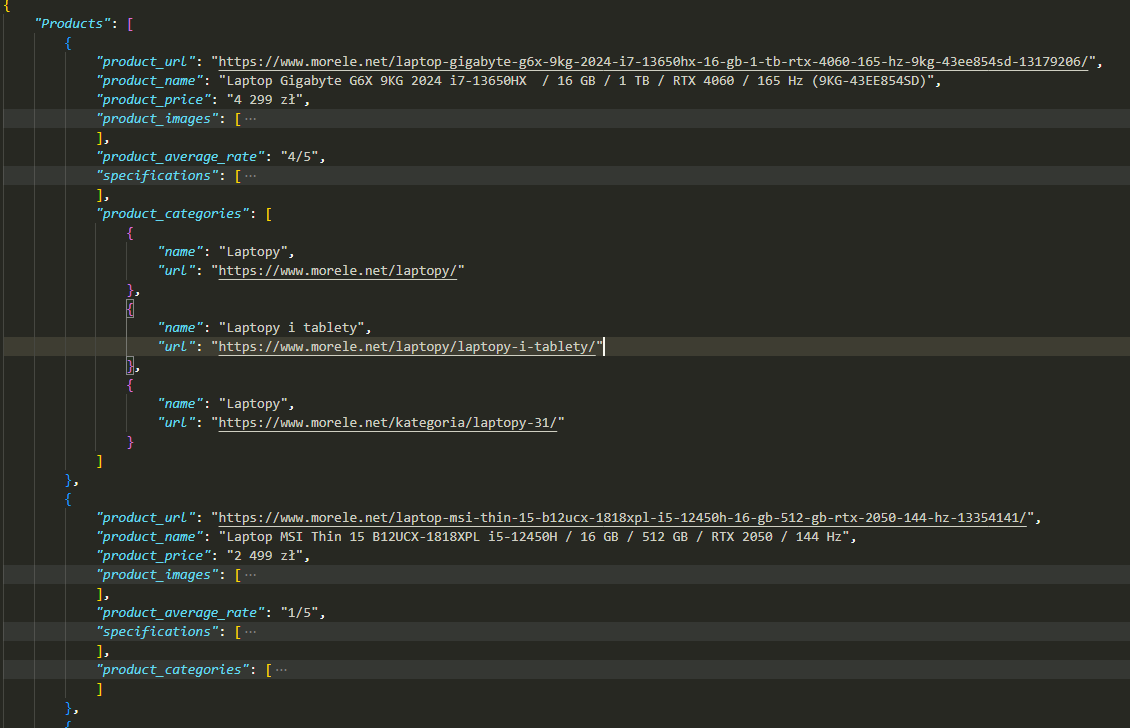
\includegraphics[width=0.9\columnwidth]{images/krzysztofBImages/products_seed.png}
    \caption{Przykładowy plik JSON z wygenerowanymi danymi produktów i kategorii}
\end{figure}
%
%
\subsubsection{Grzegorz Golonka: Formularze do modelów bazodanowych}
\label{section:1.3.23}
\textit{
Implementacja formularzy użytkownika w projekcie \texttt{kmg\_store} oraz ich integracja z widokami w celu obsługi rejestracji, logowania, adresów oraz metod płatności.
}

W ramach zadania stworzono i zaimplementowano następujące formularze:
\begin{itemize}
    \item \textbf{UserLoginForm} – formularz logowania użytkownika, obsługujący pola \texttt{email} i \texttt{password}. Formularz został zintegrowany z widokiem \texttt{UserLoginView}, umożliwiając autoryzację użytkownika oraz synchronizację danych sesji.
    \item \textbf{UserAddressForm} – formularz do zarządzania adresami użytkownika, umożliwiający zapis i odczyt danych adresowych (\texttt{street}, \texttt{city}, \texttt{postal\_code}, \texttt{country}, \texttt{is\_default}). Formularz został użyty w widokach \texttt{UserAddressCreationView} i \texttt{AddressSelectionView}, wspierając zarządzanie adresami oraz wybór domyślnego adresu dostawy.
    \item \textbf{PaymentMethodForm} – formularz obsługujący dodawanie metod płatności (karty kredytowe, Blik). Zawiera walidację wymaganych pól w zależności od wybranej metody płatności. Formularz zintegrowano z widokiem \texttt{PaymentMethodView}, umożliwiając zapis metod płatności i obsługę kodów Blik.
    \item \textbf{UserRegistrationForm (częściowo)} – formularz rejestracyjny użytkownika, obejmujący m.in. walidację unikalności e-maila oraz poprawności numeru telefonu. Formularz został zintegrowany z widokiem \texttt{UserRegisterView}, wspierając proces tworzenia konta użytkownika.
\end{itemize}

Formularze i widoki zostały zaimplementowane zgodnie z wymogami projektu, zapewniając obsługę walidacji, intuicyjny interfejs oraz integrację z modelem danych.
%
%
\subsubsection{Grzegorz Golonka: Obsługa widoków adresu i listy adresów użytkownika}
\label{section:1.3.24}
\textit{
Implementacja widoków \texttt{UserAddressCreationView} oraz \texttt{AddressSelectionView} w celu obsługi zarządzania adresami użytkownika w procesie tworzenia zamówienia.
}

Zrealizowano następujące funkcjonalności:
\begin{itemize}
    \item \textbf{Widok \texttt{UserAddressCreationView}} – umożliwia dodanie nowego adresu użytkownika z wykorzystaniem formularza \texttt{UserAddressForm}. Widok obsługuje przypisanie użytkownika do adresu, ustawianie adresu jako domyślnego oraz zapis do sesji identyfikatora wybranego adresu.
    \item \textbf{Widok \texttt{AddressSelectionView}} – umożliwia wyświetlenie listy zapisanych adresów użytkownika, wybór adresu domyślnego oraz zapis wybranego adresu do sesji w celu wykorzystania w dalszym procesie zamówienia.
\end{itemize}

Widoki wykorzystują istniejące modele \texttt{Address} oraz formularz \texttt{UserAddressForm}, zapewniając pełną spójność z wcześniej zaimplementowanymi komponentami systemu.

%
%
\subsubsection{Grzegorz Golonka: Obsługa widoków metody płatności i kodu Blik}
\label{section:1.3.25}
\textit{
Implementacja widoków \texttt{PaymentMethodView} oraz \texttt{BlikCodeView} w celu zarządzania metodami płatności użytkownika oraz obsługi płatności Blik w procesie składania zamówienia.
}

W ramach zadania zrealizowano następujące funkcjonalności:
\begin{itemize}
    \item \textbf{Widok \texttt{PaymentMethodView}} – umożliwia użytkownikowi dodanie nowej metody płatności z wykorzystaniem formularza \texttt{PaymentMethodForm}. Widok zapisuje wprowadzone dane do bazy, przypisuje je do użytkownika oraz przechowuje identyfikator metody płatności w sesji na potrzeby tworzenia zamówienia. Widok obsługuje również przekierowanie na stronę wprowadzania kodu Blik, jeśli wybrano tę metodę płatności.
    \item \textbf{Widok \texttt{BlikCodeView}} – obsługuje wprowadzanie kodu Blik przez użytkownika. Widok waliduje kod (sprawdzając poprawność długości i czy składa się wyłącznie z cyfr) oraz zapisuje go w sesji, umożliwiając dalsze wykorzystanie w procesie zamówienia.
\end{itemize}

Funkcjonalności zapewniają pełną spójność z widokami zarządzania adresem oraz procesem składania zamówienia, pozwalając na przechowywanie danych w sesji oraz ich późniejsze wykorzystanie przy tworzeniu obiektu \texttt{Order}.

%
%
\subsubsection{Grzegorz Golonka: Weryfikacja danych przy składaniu zamówienia}
\label{section:1.3.26}
\textit{
Implementacja logiki odpowiedzialnej za weryfikację danych użytkownika w procesie składania zamówienia w widoku \texttt{OrderCreateView}.
}

\paragraph{Zakres prac}
Zaimplementowano następujące elementy:
\begin{itemize}
    \item Pobieranie danych koszyka użytkownika (\texttt{Cart}) oraz sesji:
    \begin{itemize}
        \item ID adresu dostawy (\texttt{selected\_address\_id}),
        \item ID metody płatności (\texttt{selected\_payment\_method\_id}),
        \item Kod Blik (\texttt{blik\_code}).
    \end{itemize}
    \item Walidacja danych użytkownika:
    \begin{itemize}
        \item Sprawdzenie obecności koszyka i jego zawartości,
        \item Weryfikacja wybranego adresu dostawy oraz metody płatności,
        \item Dla metody płatności \texttt{Blik} sprawdzenie obecności kodu \texttt{blik\_code}.
    \end{itemize}
\end{itemize}
%
%
\subsubsection{Grzegorz Golonka: Tworzenie zamówienia i wysyłanie powiadomień}
\label{section:1.3.27}
\textit{
Implementacja logiki odpowiedzialnej za utworzenie zamówienia oraz wysyłanie powiadomień do użytkownika w widoku \texttt{OrderCreateView}.
}

\paragraph{Zakres prac}
Zaimplementowano następujące elementy:
\begin{itemize}
    \item Utworzenie zamówienia:
    \begin{itemize}
        \item Obiekt \texttt{Order} tworzony na podstawie danych koszyka, adresu dostawy i metody płatności,
        \item Dodanie produktów do zamówienia na podstawie zawartości koszyka,
        \item Usunięcie zawartości koszyka po utworzeniu zamówienia,
        \item Zapisanie ID zamówienia w sesji użytkownika (\texttt{current\_order\_id}).
    \end{itemize}
    \item Powiadomienia:
    \begin{itemize}
        \item Wysłanie powiadomienia e-mail z potwierdzeniem zamówienia przy użyciu funkcji \texttt{send\_order\_confirmation\_email},
        \item Wiadomość zawiera szczegóły zamówienia, takie jak lista produktów, metoda płatności oraz adres dostawy.
    \end{itemize}
\end{itemize}
%
%
\subsubsection{Grzegorz Golonka: Implementacja widoku szczegółów zamówienia}
\label{section:1.3.28}
\textit{
Stworzenie widoku \texttt{OrderDetailView}, umożliwiającego użytkownikowi przegląd szczegółów zamówienia.
}
Zaimplementowano następujące elementy:
\begin{itemize}
    \item \textbf{Widok \texttt{OrderDetailView}:}
    \begin{itemize}
        \item Pobieranie zamówienia przypisanego do zalogowanego użytkownika,
        \item Obsługa widoku administracyjnego z możliwością przeglądu wszystkich zamówień,
        \item Przekazanie danych o zamówieniu do kontekstu, w tym:
        \begin{itemize}
            \item Lista produktów w zamówieniu,
            \item Informacje o statusie zamówienia,
            \item Możliwość oceniania produktów po zakończeniu dostawy.
        \end{itemize}
    \end{itemize}
    \item \textbf{Szablon \texttt{order\_detail.html}:}
    \begin{itemize}
        \item Wyświetlanie szczegółów zamówienia, takich jak:
        \begin{itemize}
            \item ID zamówienia, status, kwota, adres dostawy, metoda płatności,
            \item Produkty w zamówieniu z odnośnikami do szczegółów produktów.
        \end{itemize}
        \item Wyświetlanie postępu realizacji zamówienia w formie graficznej (\textit{stepper}).
    \end{itemize}
\end{itemize}
%
%
\subsubsection{Grzegorz Golonka: Automatyczna aktualizacja statusu zamówienia}
\label{section:1.3.29}
\textit{
Implementacja logiki odpowiedzialnej za automatyczną aktualizację statusu zamówienia oraz jej symulację.
}
Zaimplementowano następujące elementy:
\begin{itemize}
    \item \textbf{Signal \texttt{post\_save}:}
    \begin{itemize}
        \item Symulacja zmiany statusu zamówienia przy jego tworzeniu,
        \item Kolejne statusy: \texttt{processing}, \texttt{in\_delivery}, \texttt{ready\_for\_pickup}, \texttt{completed},
        \item Zmiana statusu co określony interwał czasowy (4–5 sekund).
    \end{itemize}
    \item \textbf{Signal \texttt{pre\_save}:}
    \begin{itemize}
        \item Śledzenie poprzedniego statusu zamówienia,
        \item Umożliwienie reakcji na zmianę statusu w przyszłych funkcjonalnościach.
    \end{itemize}
    \item \textbf{Obsługa dynamicznej aktualizacji:}
    \begin{itemize}
        \item Skrypt \texttt{order\_detail.js} cyklicznie sprawdzający status zamówienia za pomocą \texttt{AJAX},
        \item Automatyczne odświeżanie widoku w przypadku zmiany statusu.
    \end{itemize}
\end{itemize}
%
%
\subsubsection{Grzegorz Golonka: Przygotowanie do oceniania produktów w zamówieniu}
\label{section:1.3.30}
\textit{
Stworzenie funkcjonalności umożliwiającej użytkownikowi ocenianie produktów w zamówieniu po jego zakończeniu.
}
Zaimplementowano następujące elementy:
\begin{itemize}
    \item \textbf{Widok \texttt{OrderDetailView}:}
    \begin{itemize}
        \item Dodanie informacji o możliwości oceniania produktów (\texttt{can\_rate}) w zależności od statusu zamówienia (\texttt{completed}).
    \end{itemize}
    \item \textbf{Szablon \texttt{order\_detail.html}:}
    \begin{itemize}
        \item Sekcja oceniania produktów:
        \begin{itemize}
            \item Formularz oceny dla każdego produktu (\texttt{value}, \texttt{comment}),
            \item Dynamiczne przyciski reakcji (lajki).
        \end{itemize}
        \item Placeholder informujący, że ocena produktów będzie dostępna po zakończeniu zamówienia.
    \end{itemize}
    \item \textbf{Skrypt \texttt{order\_detail.js}:}
    \begin{itemize}
        \item Obsługa wysyłania ocen za pomocą formularza,
        \item Walidacja pól oceny (\texttt{value} w zakresie 1–5, \texttt{comment}),
        \item Komunikaty o sukcesie lub błędach podczas przesyłania danych.
    \end{itemize}
\end{itemize}
%
%
%
\subsubsection{Grzegorz Golonka: Automatyczne tworzenie konwersacji przy zamówieniu}
\label{section:1.3.31}
\textit{
Implementacja automatycznego tworzenia konwersacji w momencie utworzenia zamówienia oraz ich aktualizacji przy zmianie statusu.
}
Zaimplementowano następujące elementy:
\begin{itemize}
    \item \textbf{Signal \texttt{post\_save}:}
    \begin{itemize}
        \item Tworzenie konwersacji związanej z zamówieniem (\texttt{status\_conversation}) po utworzeniu obiektu \texttt{Order}.
        \item Dodawanie uczestników do konwersacji (użytkownik składający zamówienie).
        \item Automatyczne generowanie wiadomości systemowej z informacją o utworzeniu zamówienia oraz jego statusie.
        \item Obsługa aktualizacji konwersacji w przypadku zmiany statusu zamówienia:
        \begin{itemize}
            \item Porównanie aktualnego i poprzedniego statusu zamówienia,
            \item Wysłanie wiadomości systemowej z informacją o zmianie statusu.
        \end{itemize}
    \end{itemize}
\end{itemize}
%
%
\subsubsection{Grzegorz Golonka: Widok listy wiadomości i konwersacji}
\label{section:1.3.32}
\textit{
Implementacja widoku wyświetlającego listę konwersacji użytkownika oraz ich podstawowych informacji.
}
Zaimplementowano następujące elementy:
\begin{itemize}
    \item \textbf{Widok \texttt{MessagesListView}:}
    \begin{itemize}
        \item Pobieranie konwersacji przypisanych do zalogowanego użytkownika.
        \item Dla administratorów:
        \begin{itemize}
            \item Wyświetlanie wszystkich konwersacji użytkowników z informacją o uczestniku i zamówieniu.
        \end{itemize}
        \item Dla użytkowników:
        \begin{itemize}
            \item Wyświetlanie konwersacji użytkownika (statusowych oraz z administratorem).
        \end{itemize}
        \item Informacja o ostatnio otwartej konwersacji użytkownika.
    \end{itemize}
    \item \textbf{Szablon \texttt{message\_list.html}:}
    \begin{itemize}
        \item Lista konwersacji po lewej stronie, z możliwością wyboru aktywnej konwersacji,
        \item Obszar wiadomości po prawej stronie, dynamicznie ładowany po wyborze konwersacji.
    \end{itemize}
\end{itemize}
%
%
\subsubsection{Grzegorz Golonka: Obsługa ładowania wiadomości}
\label{section:1.3.33}
\textit{
Implementacja widoku i logiki odpowiedzialnej za dynamiczne ładowanie wiadomości w wybranej konwersacji.
}
Zaimplementowano następujące elementy:
\begin{itemize}
    \item \textbf{Widok \texttt{load\_messages}:}
    \begin{itemize}
        \item Pobieranie wszystkich wiadomości przypisanych do wybranej konwersacji.
        \item Zaktualizowanie informacji o ostatnio otwartej konwersacji w profilu użytkownika.
        \item Zwracanie wiadomości w formacie \texttt{JSON}, zawierającym:
        \begin{itemize}
            \item Treść wiadomości,
            \item Nadawcę,
            \item Czas wysłania wiadomości.
        \end{itemize}
    \end{itemize}
    \item \textbf{Skrypt \texttt{handle\_messages.js}:}
    \begin{itemize}
        \item Dynamiczne ładowanie wiadomości dla aktywnej konwersacji po stronie klienta.
        \item Obsługa przewijania listy wiadomości na dół po załadowaniu.
    \end{itemize}
\end{itemize}
%
%
\subsubsection{Grzegorz Golonka: Utworzenie systemu oceniania produktów}
\label{section:1.3.34}
\textit{
Implementacja systemu oceniania produktów, umożliwiającego użytkownikom dodawanie i aktualizowanie ocen oraz komentarzy.
}
Zaimplementowano następujące elementy:
\begin{itemize}
    \item \textbf{Model \texttt{Rate}:}
    \begin{itemize}
        \item Relacja wiele-do-jednego z modelem \texttt{User} oraz \texttt{Product}.
        \item Pola:
        \begin{itemize}
            \item \texttt{value} – wartość oceny (1–5),
            \item \texttt{comment} – opcjonalny komentarz,
            \item \texttt{created\_at} – data utworzenia oceny.
        \end{itemize}
        \item Metoda \texttt{can\_edit}, sprawdzająca, czy użytkownik może edytować daną ocenę.
    \end{itemize}
    \item \textbf{Widok \texttt{rate\_product}:}
    \begin{itemize}
        \item Obsługa żądań \texttt{POST} dla dodawania i aktualizowania ocen.
        \item Walidacja danych:
        \begin{itemize}
            \item Sprawdzenie poprawności wartości oceny (\texttt{1–5}),
            \item Walidacja autoryzacji użytkownika.
        \end{itemize}
        \item Aktualizacja średniej oceny produktu po każdej zmianie.
    \end{itemize}
\end{itemize}
%
%
\subsubsection{Grzegorz Golonka: Integracja systemu ocen z widokiem produktu}
\label{section:1.3.35}
\textit{
Integracja systemu oceniania z widokiem szczegółów zamówienia i widokiem produktu, umożliwiająca użytkownikom przeglądanie i edytowanie ocen.
}
Zaimplementowano następujące elementy:
\begin{itemize}
    \item \textbf{Widok \texttt{OrderDetailView}:}
    \begin{itemize}
        \item Dodanie możliwości oceniania produktów z poziomu szczegółów zamówienia (\texttt{can\_rate}).
        \item Formularz dodawania oceny z polami:
        \begin{itemize}
            \item \texttt{value} – wartość oceny,
            \item \texttt{comment} – komentarz.
        \end{itemize}
    \end{itemize}
    \item \textbf{Widok \texttt{ProductDetailView}:}
    \begin{itemize}
        \item Wyświetlanie listy ocen produktu z możliwością ich edycji przez autora.
        \item Formularz edycji oceny z dynamicznym wczytywaniem istniejących danych.
    \end{itemize}
    \item \textbf{Szablony:}
    \begin{itemize}
        \item \texttt{order\_detail.html} – formularz oceniania dostępny w szczegółach zamówienia.
        \item \texttt{product\_detail.html} – lista ocen z obsługą gwiazdek, komentarzy oraz formularza edycji.
    \end{itemize}
\end{itemize}
%
%
\subsubsection{Grzegorz Golonka: Dynamiczna obsługa ocen i ich edycji}
\label{section:1.3.36}
\textit{
Wdrożenie mechanizmów dynamicznej obsługi ocen produktów, umożliwiających aktualizację ocen i komentarzy w czasie rzeczywistym.
}
Zaimplementowano następujące elementy:
\begin{itemize}
    \item \textbf{Skrypt \texttt{order\_detail.js}:}
    \begin{itemize}
        \item Obsługa wysyłania formularza ocen:
        \begin{itemize}
            \item Walidacja danych,
            \item Wysłanie żądania AJAX do widoku \texttt{rate\_product}.
        \end{itemize}
        \item Automatyczne odświeżanie danych w widoku po dodaniu nowej oceny.
    \end{itemize}
    \item \textbf{Skrypt \texttt{product\_detail.js}:}
    \begin{itemize}
        \item Obsługa wyświetlania formularza edycji oceny:
        \begin{itemize}
            \item Pobieranie istniejących danych oceny (gwiazdki, komentarz),
            \item Dynamiczne generowanie formularza edycji na stronie.
        \end{itemize}
        \item Obsługa aktualizacji danych oceny:
        \begin{itemize}
            \item Wysłanie żądania AJAX do widoku \texttt{rate\_product},
            \item Dynamiczna aktualizacja danych oceny na stronie po ich zapisaniu.
        \end{itemize}
    \end{itemize}
    \item \textbf{Widok \texttt{get\_ratings\_html}:}
    \begin{itemize}
        \item Generowanie HTML z listą ocen dla produktu.
        \item Obsługa dynamicznego odświeżania sekcji ocen na stronie.
    \end{itemize}
\end{itemize}
%
%

\subsubsection{Karol Woźniak: zadanie nr 2}
\textit{Krótkie wyjaśnienie, opis lub odwołanie do załącznika.}

\subsection{Załączniki}
\textit{Lista załączników lub dodatkowych materiałów potwierdzających zrealizowane zadania.}

% --------------------------------------------------------------------
%%%%%%% odkomentować gdy bibliografia ma być wewnątrz dokumentu
% --------------------------------------------------------------------
%\begin{thebibliography}{11}
%
%\addcontentsline{toc}{section}{Literatura}
%
%\bibitem{ZAN}
%C. Zannoni and P. Pasini, 
%\emph{Advances in the Computer Simulatons of Liquid Crystals}, Kluwer Academic Publishers, 2000.
%
%\end{thebibliography}

\end{document}

